
\documentclass[a4paper,11pt]{article}%,twocolumn
%% packages

\usepackage{blindtext} % needed for creating dummy text passages
%\usepackage{ngerman} % needed for German default language
\usepackage{amsmath} % needed for command eqref
\usepackage{amssymb} % needed for math fonts
\usepackage[colorlinks=true,breaklinks]{hyperref} % needed for creating hyperlinks in the document, the option colorlinks=true gets rid of the awful boxes, breaklinks breaks lonkg links (list of figures), and ngerman sets everything for german as default hyperlinks language
\usepackage[hyphenbreaks]{breakurl} % ben�tigt f�r das Brechen von URLs in Literaturreferenzen, hyphenbreaks auch bei links, die �ber eine Seite gehen (mit hyphenation).
\usepackage{xcolor}
\definecolor{c1}{rgb}{0,0,1} % blue
\definecolor{c2}{rgb}{0,0.3,0.9} % light blue
\definecolor{c3}{rgb}{0.3,0,0.9} % red blue
\hypersetup{
    linkcolor={c1}, % internal links
    citecolor={c2}, % citations
    urlcolor={c3} % external links/urls
}
%\usepackage{cite} % needed for cite
\usepackage[square,authoryear]{natbib} % needed for cite and abbrvnat bibliography style
\usepackage[nottoc]{tocbibind} % needed for displaying bibliography and other in the table of contents
\usepackage{graphicx} % needed for \includegraphics 
\usepackage{longtable} % needed for long tables over pages
\usepackage{bigstrut} % needed for the command \bigstrut
\usepackage{enumerate} % needed for some options in enumerate
%\usepackage{todonotes} % needed for todos
\usepackage{makeidx} % needed for creating an index
\makeindex
\usepackage{gensymb}
\usepackage{url}
\usepackage{psfrag}
\usepackage{multirow}
\usepackage{subfigure}
%% page settings

\usepackage[top=20mm, bottom=20mm,left=15mm,right=15mm]{geometry} % needed for page border settings
\parindent=0mm % for space of first line of new text block
\sloppy % for writing with hyphenless justification (tries to)
\hyphenation{} % use hyphenation of tolerance parametershttp://www.jr-x.de/publikationen/latex/tipps/zeilenumbruch.html
\hyphenpenalty=10000
\exhyphenpenalty=10000
\usepackage{fancyhdr} % needed for head and foot options
%% my macros

%% Text fomats
\newcommand{\tbi}[1]{\textbf{\textit{#1}}}

%% Math fonts
\newcommand{\bbA}{\mathbb{A}}
\newcommand{\bbB}{\mathbb{B}}
\newcommand{\bbC}{\mathbb{C}}
\newcommand{\bbD}{\mathbb{D}}
\newcommand{\bbE}{\mathbb{E}}
\newcommand{\bbF}{\mathbb{F}}
\newcommand{\bbG}{\mathbb{G}}
\newcommand{\bbH}{\mathbb{H}}
\newcommand{\bbI}{\mathbb{I}}
\newcommand{\bbJ}{\mathbb{J}}
\newcommand{\bbK}{\mathbb{K}}
\newcommand{\bbL}{\mathbb{L}}
\newcommand{\bbM}{\mathbb{M}}
\newcommand{\bbN}{\mathbb{N}}
\newcommand{\bbO}{\mathbb{O}}
\newcommand{\bbP}{\mathbb{P}}
\newcommand{\bbQ}{\mathbb{Q}}
\newcommand{\bbR}{\mathbb{R}}
\newcommand{\bbS}{\mathbb{S}}
\newcommand{\bbT}{\mathbb{T}}
\newcommand{\bbU}{\mathbb{U}}
\newcommand{\bbV}{\mathbb{V}}
\newcommand{\bbW}{\mathbb{W}}
\newcommand{\bbX}{\mathbb{X}}
\newcommand{\bbY}{\mathbb{Y}}
\newcommand{\bbZ}{\mathbb{Z}}
\usepackage[ framed, numbered]{matlab-prettifier}%framed,%
\usepackage{listings}
\usepackage{physics}
\usepackage{pdfpages}
\usepackage[toc,page]{appendix}
\usepackage{float}
\usepackage{pifont}


\begin{document}
\begin{titlepage}
\center % Center everything on the page

%-------------------------------------------------------------------------------------
%	HEADING SECTIONS
%------------------------------------------------------------------------------------
\textbf{\large Department of Electrical and Computer Engineering}\\[0.5cm]
\textbf{\Large University of Colorado at Boulder}\\[1cm]
\textbf{\large ECEN5730 - Practical PCB design}\\[2cm]

\includegraphics[width=0.3\textwidth]{figures/cu}\\[2cm] 

	
%-------------------------------------------------------------------------------------
%	TITLE SECTION
%------------------------------------------------------------------------------------

\textbf{\Huge Board Good Layout/Bad Layout }\\[0.2cm]

\textbf{\Large Report}\\[2cm]
\vspace{1.5cm}
\begin{figure}[H]
	\centering
	
\includegraphics[scale=0.2]{figures/qr_download.png}
	\label{555_schematic}
\end{figure}\vspace{1.5cm}


%----------------------------------------------------------------------------------------
%	MEMBERS SECTION
%----------------------------------------------------------------------------------------


\vfill

\textbf{\large Submitted by}

{\large Parth Thakkar}\\[0.5cm]




%----------------------------------------------------------------------------------------
%	DATE SECTION
%----------------------------------------------------------------------------------------

\textbf{\large Submitted on}\\
\textbf{\Large \today} % Date, change the \today to a set date if you want to be precise

%----------------------------------------------------------------------------------------

\vfill % Fill the rest of the page with whitespace

\end{titlepage}

\pagebreak

\tableofcontents
\listoffigures
\listoftables
\vfill
\begin{center}
	\textbf{\textit{*PDF is clickable}}
\end{center}

\pagebreak

\section{Introduction}


This lab aims to teach students how to design and build a working electronic device from start to finish. The main objective is to provide hands-on experience in the different steps involved in creating a prototype.\\

we start by drawing a simple diagram of the circuit they want to build on a piece of paper. Then creating the PCB in altium designer\\

After building the board, test it to make sure it works as planned. Use tools like multimeters and oscilloscopes to measure voltages and signals. If something doesn't work right, figure out what's wrong and fix it.\\

\textbf{Measurements to be Conducted:}

\begin{enumerate}
	\item \textbf{Oscilloscope Analysis:} Use an oscilloscope equipped with a 10x probe to observe the rise time fall time of switching noise on the power rail due to switching of pins
	\item \textbf{Noise Measurement:} Examine the noise on power rail with slammer circuit to see difference between held high pin with software and local power
	\item \textbf{current measurement:} measure the current going thorough slammer 10ohm resistor.
	\item \textbf{current measurement:} measure the current going thorough slammer 47ohm resistor.
\end{enumerate}

For the construction, 1206 size surface-mount device (SMD) components were chosen and soldered onto a printed circuit board (PCB).

\section{Project Plan}
\begin{enumerate}
	\item Using Micro B usb instead of Mini B
	\item Integrate an external power source connector for a 5V AC to DC adapter to supply power to the circuit board.
	\item Implement a voltage converter to step down from 5V to 3.3V using LDO.
	\item Functionality to measure the in-rush current.
	\item Design header layout in such a way that it could be compatable with all the arduino shields.
	\item Use isolation of circuit with three pin switches
	\item Use as less cross under as possible without making size bigger
	\item Employ red LEDs and 50 ohm resistors as loads for three of the switch outputs from each hex inverter.
	\item Calculate the current consumption of slammer 50 ohm resistor.
	\item Use same size of commercial Layouts.
	\item Design one side of the printed circuit board (PCB) using optimal layout practices and the opposite side with suboptimal layout techniques. In the less effective layout, position the decoupling capacitors significantly away from the Vcc pin.
	\item  Ensure consistent component placement and routing across both sections of the PCB, with the exception of the decoupling capacitor's positioning.
	\item  Establish test points for the following signals:
	      \begin{itemize}
		      \item 5V test point
		      \item test point at 3.3V
		      \item Voltage across D+ pin of usb
		      \item Voltage across SCL line
		      \item Voltage across arduino RX
		      \item Voltage across arduino TX
	      \end{itemize}

	\item Add a decoupling capacitor for the Atmega328P IC to mitigate switching noise.
	\item Add a Ferrite Bead (LC low pass filter) to Analog Reference for the Atmega328P.
	\item Implement a copper pour for the ground plane to enhance circuit stability.
	\item Incorporate indicator lights, testing points, and isolation switches for comprehensive functionality and diagnostic capabilities.
\end{enumerate}



\section{Risk Management}
\begin{enumerate}
	\item Signal lines will have a width of 6 mils to maintain signal integrity.
	\item Power lines will be designed with a width of 20 mils to distinguish them easily and support adequate current flow.
	\item Test points will be strategically placed and clearly labeled for easy identification.
	\item Isolation switches will be installed at each stage to facilitate troubleshooting and debugging.
	\item Use appropriate voltage regulators (e.g., AMS1117) to provide stable and regulated power to the components.
	\item Include sufficient decoupling capacitors near power pins of ICs to minimize noise and ensure stable power delivery.
	\item Use a TVS diode (SRV05-4) to protect against voltage spikes and transients.
	\item Select a reliable USB to Serial converter (e.g., CH340G) with good driver support.
	\item Ensure proper routing of USB data lines (D+ and D-) to minimize signal integrity issues.
	\item Provide sufficient ground connections and shielding to reduce noise and interference on USB lines
	\item Choose appropriate crystal oscillators (e.g., 16MHz and 12MHz) based on the requirements of the microcontroller and CH340 components and add load resistor for high impedance.
	\item Place the crystal oscillators close to the microcontroller to minimize trace lengths and ensure stable clock signals.
	\item Design the PCB layout with manufacturability in mind, following design rules and guidelines provided by the PCB manufacturer.
	\item Use standard component packages and footprints to ensure compatibility with assembly processes.
	      Provide clear and concise assembly instructions, including component placement, orientation, and soldering guidelines.
\end{enumerate}


\section{Block Diagram, Schematic and Layout}
\subsection{Block Diagram}

\begin{figure}[H]
	\centering
	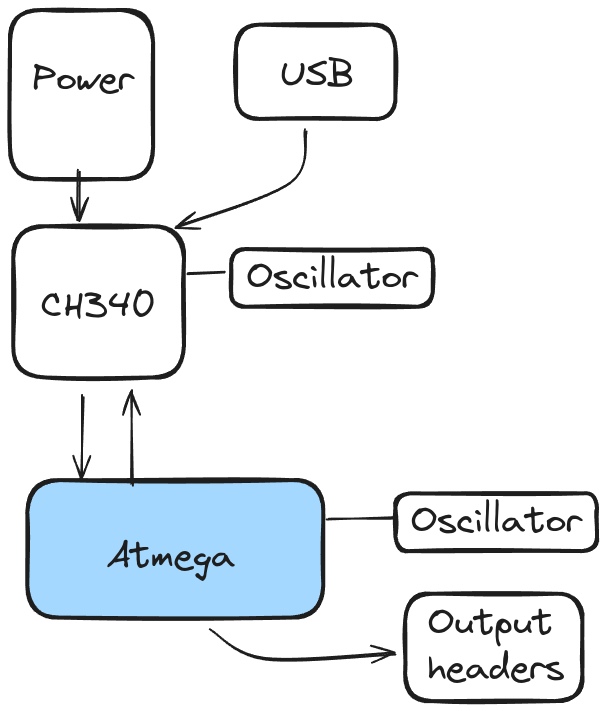
\includegraphics[scale=0.4]{figures/blockdiagram.png}
	\caption{Block diagram for Golder arduino}
\end{figure}

\begin{enumerate}
	\item Power: This block represents the power supply for the system. It provides the necessary voltage and current to power the other components.
	\item USB: The USB block indicates that the system can be connected to a computer or other devices via a USB port. This connection can be used for power supply, data transfer, or programming the microcontroller.
	\item CH340: The CH340 is a USB to serial converter chip. It facilitates communication between the USB port and the microcontroller by converting USB signals to serial signals and vice versa.
	\item Atmega: This block represents the Atmega microcontroller, which is the main processing unit of the system. It executes the programmed instructions and interacts with other components.
	\item Oscillator: The system includes two oscillator blocks. Oscillators provide the clock signal required for the microcontroller and other components to operate at a specific frequency. The presence of two oscillators suggests that the system may use different clock frequencies for different purposes.
	\item Output headers: The output headers block indicates that the system has connectors or pins that allow it to interface with external devices or peripherals. These headers can be used to send or receive signals, control other devices, or expand the functionality of the system.
\end{enumerate}


\subsection{Component listings}
\begin{table}[H]
	\centering
	\caption{Component List for Board 3}
	\begin{tabular}{|c|c|c|}
		\hline
		\textbf{Item No.} & \textbf{Component}                       & \textbf{Part Number/Value}                 \\\hline
		1                 & Microcontroller                          & Atmega328P-ANR                             \\\hline
		2                 & USB to Serial Converter                  & CH340G                                     \\\hline
		3                 & Crystal Oscillators                      & 16MHz (X322516MLB4SI),                     \\\hline
		3                 & Crystal Oscillators                      & 12MHz (X322512MSB4SI),                     \\\hline
		4                 & Voltage Regulator (LDO)                  & AMS1117                                    \\\hline
		5                 & Transient Voltage Suppressor (TVS) Diode & SRV05-4                                    \\\hline
		6                 & Resistors                                & Various values (not specified)             \\\hline
		7                 & Capacitors                               & Decoupling capacitors                      \\\hline
		8                 & Connectors                               & Power jack,                                \\ \hline
		9                 & USB                                      & USB mini connector                         \\ \hline
		10                & Output Headers                           & Header pins (male and female)              \\\hline
		11                & Switch                                   & Power selector switch                      \\\hline
		12                & LEDs                                     & Indicator LEDs for 5V and 3.3V power rails \\\hline
	\end{tabular}
	\label{tab:component_list}
\end{table}



\subsection{Schematic Overview}


\begin{figure}[H]
	\centering
	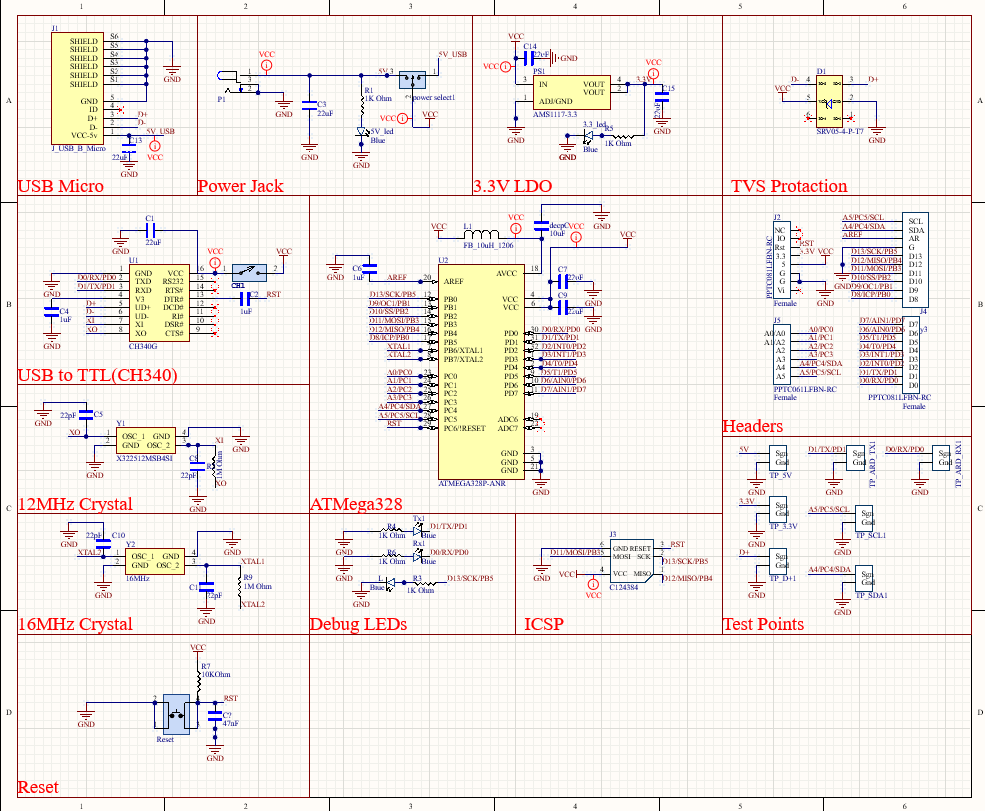
\includegraphics[scale=0.5]{figures/schematic.png}
	\caption{Schematic}
\end{figure}

\begin{enumerate}
	\item \textbf{Power Supply:}\\
	      I will be using USB micro B for the power USB instead of USB mini B\\

	      The schematic includes two power input options: a USB Micro connector and a power jack. The USB Micro connector allows the system to be powered through a USB connection, while the power jack enables the use of an external power supply. The power source selection is controlled by a switch, which determines whether the system is powered via USB or the external power jack.\\

	      The incoming power is then regulated using a 3.3V LDO (Low Dropout) voltage regulator. The LDO takes the input voltage (either from USB or the power jack) and steps it down to a stable 3.3V, which is used to power the microcontroller and other components in the system. The LDO ensures a clean and regulated power supply, minimizing noise and voltage fluctuations.

	\item \textbf{USB to TTL (CH340):}\\The schematic includes a USB to TTL converter based on the CH340 chip. This subsystem enables serial communication between the microcontroller and a computer or other USB host. The CH340 chip converts USB signals to TTL (Transistor-Transistor Logic) levels and vice versa, allowing the microcontroller to communicate with the USB host.\\

	      The USB data lines (D+ and D-) are connected to the CH340 chip, which handles the USB protocol and data transfer. The chip also provides the necessary signals for USB enumeration and handshaking. The converted TTL signals (RX and TX) are then connected to the corresponding pins of the microcontroller for serial communication.
	\item \textbf{Microcontroller (ATMega328):}\\
	      The heart of the system is the ATMega328 microcontroller. It is a powerful 8-bit microcontroller from the AVR family, widely used in Arduino boards. The microcontroller is responsible for executing the programmed instructions, controlling peripherals, and managing the overall functionality of the system.\\

	      The schematic shows the ATMega328 with its various pin connections. The power pins (VCC and GND) are connected to the regulated 3.3V supply and ground, respectively. The ICSP (In-Circuit Serial Programming) header is provided for programming the microcontroller using an external programmer.
	\item \textbf{Oscillators:}\\
	      The schematic includes two crystal oscillators: a 16MHz crystal and a 12MHz crystal. These oscillators provide the necessary clock signals for the microcontroller and other timing-dependent components. The 16MHz crystal is the primary clock source for the ATMega328, determining its operating speed and timing characteristics. The 12MHz crystal may be used for other purposes or as an alternative clock source if required.\\

	      The oscillators are connected to the corresponding pins of the microcontroller (XTAL1 and XTAL2) along with the necessary load capacitors. The load capacitors help to stabilize the oscillator's frequency and ensure reliable operation.
	\item \textbf{Debug LEDs:}\\
	      The schematic includes two debug LEDs connected to the microcontroller. These LEDs are useful for visual feedback and debugging purposes during development. They can be controlled by the microcontroller to indicate various states, errors, or progress of the system.\\

	      The LEDs are connected to the microcontroller's GPIO (General Purpose Input/Output) pins through current-limiting resistors. The resistors ensure that the LEDs operate within their specified current ratings and protect the microcontroller's pins from excessive current draw.
	\item \textbf{ICSP (In-Circuit Serial Programming):}\\
	      The ICSP header provides a means to program the microcontroller using an external programmer. It allows for direct access to the microcontroller's programming interface, enabling firmware updates, debugging, and initial programming.\\

	      The ICSP header includes the necessary pins for programming, such as MOSI (Master Out Slave In), MISO (Master In Slave Out), SCK (Serial Clock), and RESET. These pins are connected to the corresponding pins of the microcontroller, allowing the programmer to communicate with the microcontroller and transfer the program code.
	\item \textbf{Test Points:}\\
	      The schematic includes several test points strategically placed at various locations. Test points are small pads or connectors that provide access to specific signals or voltages for testing and measurement purposes. They allow developers to easily probe and monitor the system's behavior during development and debugging.\\

	      The test points in this schematic are connected to important signals such as the power supply voltages (3.3V and GND), the ICSP signals (SCK, MOSI, MISO), and the serial communication signals (RX and TX). These test points facilitate the use of oscilloscopes, logic analyzers, or multimeters to analyze and troubleshoot the system.
\end{enumerate}


\subsection{Layout Considerations}
For the PCB layout, several factors are critical:

\begin{enumerate}
	\item \textbf{Test Probes:} Designated points for measuring power rail voltage, the output from the 555 timer, and the voltage across a 1k resistor. Each test point is accessible via individual switches for isolation.
	\item \textbf{Decoupling Capacitor and Ferrite bead:} Positioned as close to the ATMega328 timer IC as possible to minimize switching noise and stabilize the power supply to the IC.
	\item \textbf{Ground Pour:} Implementing a ground pour around signal and power traces to enhance signal integrity and provide a better return path for signals, reducing interference and improving circuit performance.
\end{enumerate}


\pagebreak
\section{Manufacturing and Assembly}

Breadboard Implementation:


\begin{figure}[H]
	\centering
	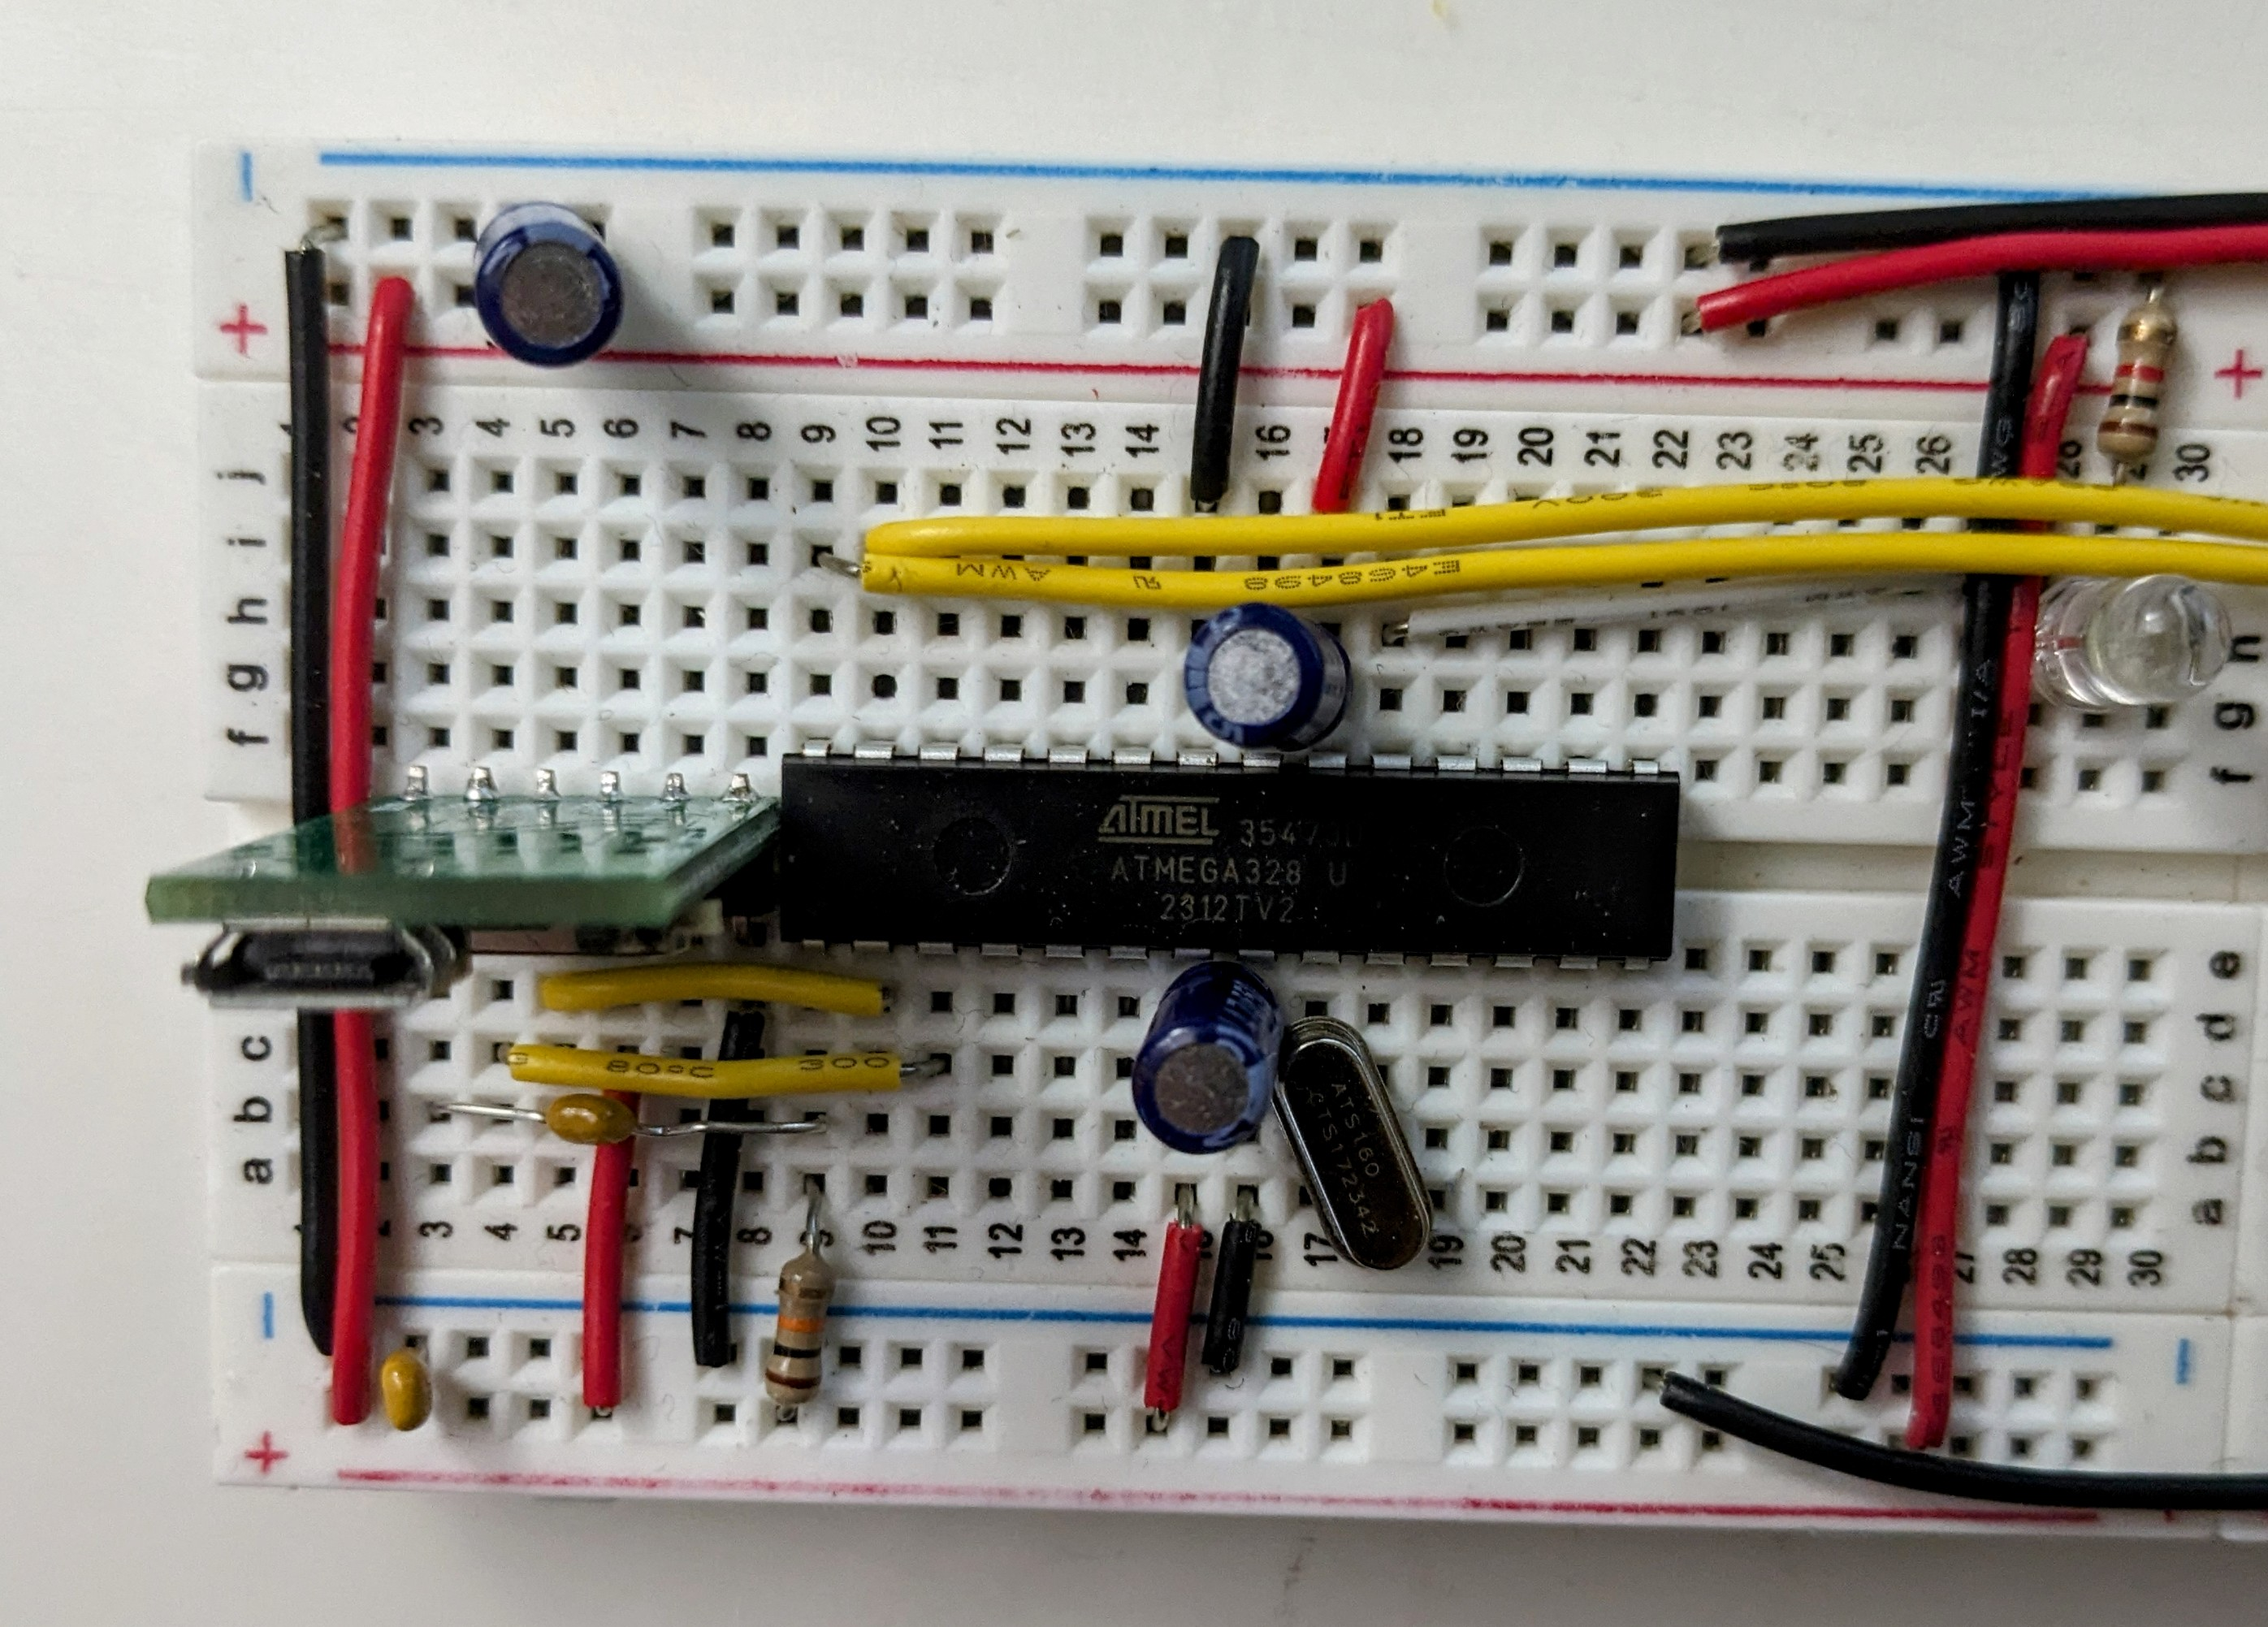
\includegraphics[scale=0.15]{figures/breadboard.jpg}
	\caption{Breadboard Implementation for Golder arduino board}
\end{figure}


\begin{figure}[H]
	\centering
	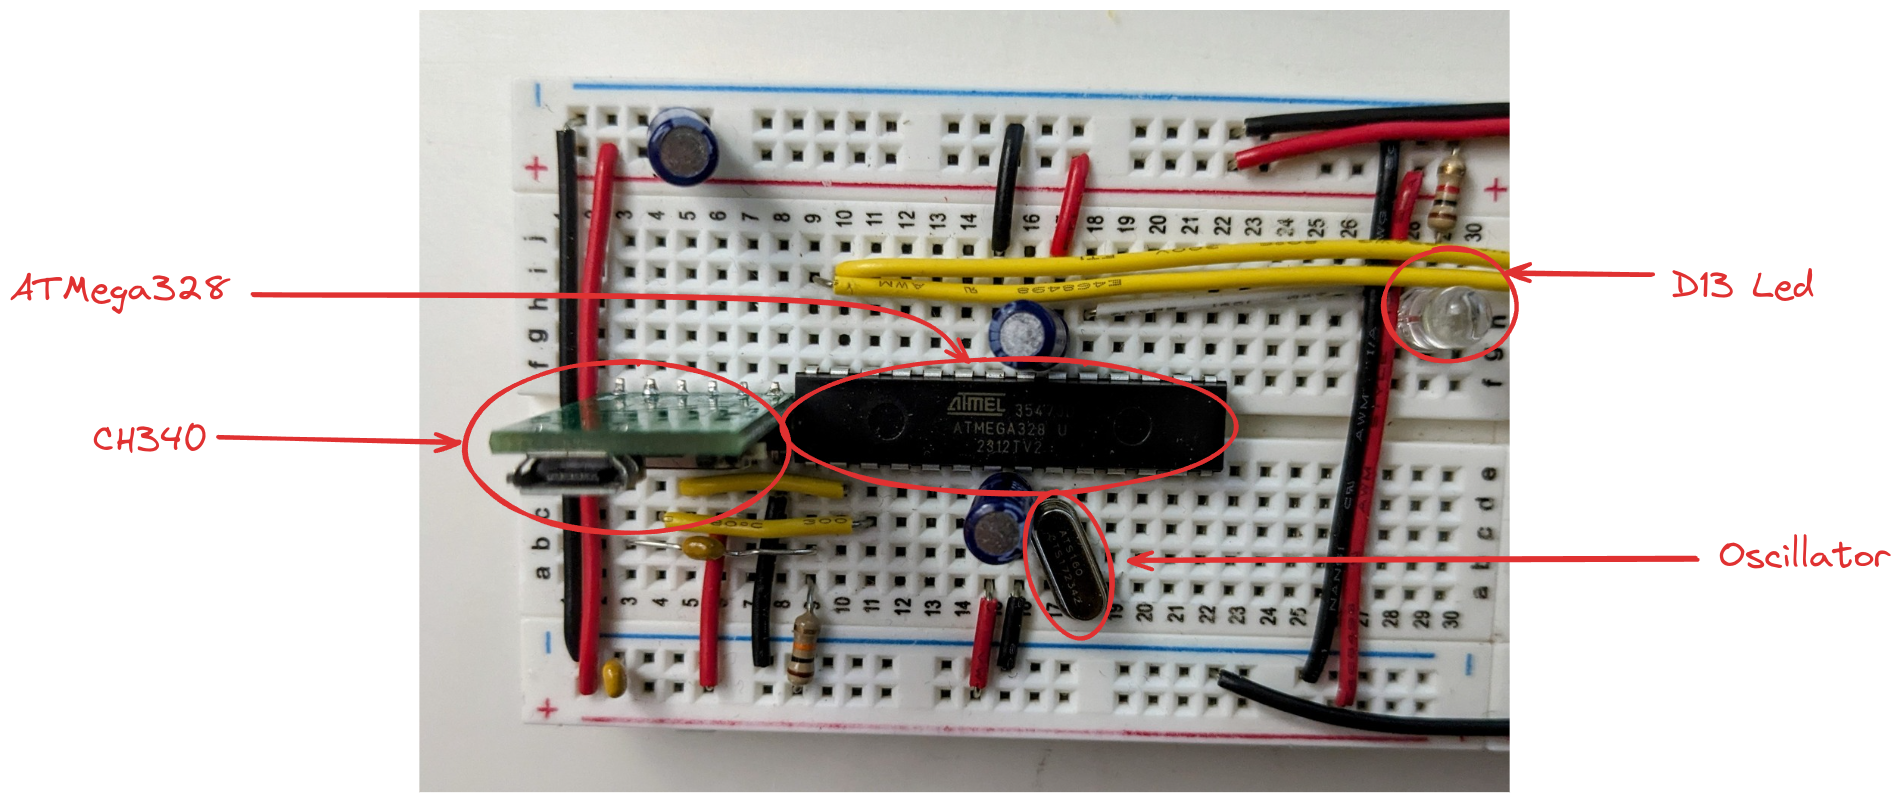
\includegraphics[scale=0.25]{figures/breadboard_des.png}
	\caption{Breadboard Implementation details}
\end{figure}


The PCB design considerations mentioned should be followed during the manufacturing and assembly process to ensure the final product meets the intended specifications and performs as designed in practical applications.\\

Here is the PCB design:\\
\begin{figure}[H]
	\centering
	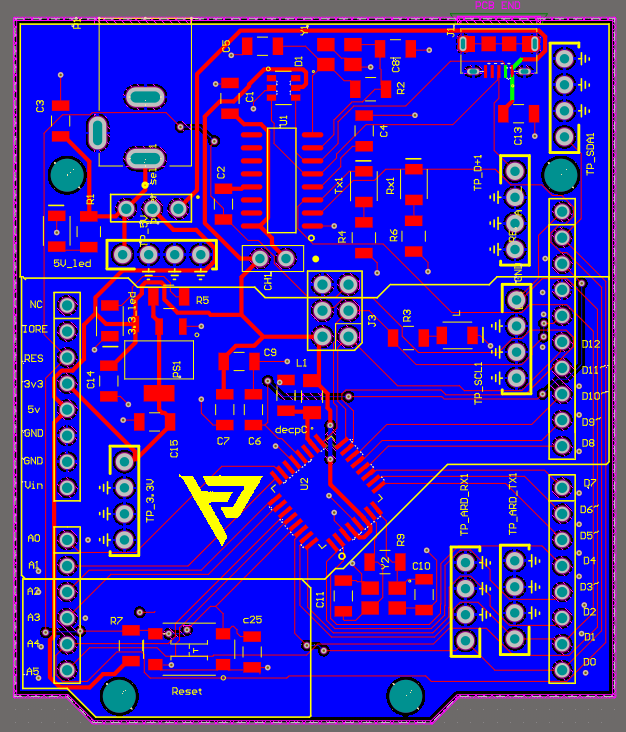
\includegraphics[scale=0.6]{figures/pcb/overall_pcb.png}
	\caption{Over all PCB}
	\label{top}
\end{figure}

\begin{figure}[H]
	\centering
	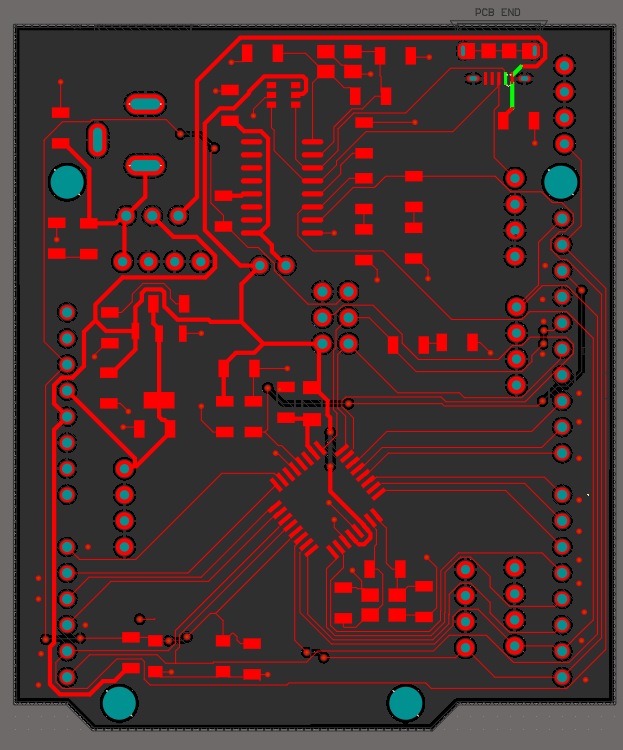
\includegraphics[scale=0.6]{figures/pcb/top_layer.png}
	\caption{Top layer}
	\label{top}
\end{figure}

\begin{figure}[H]
	\centering
	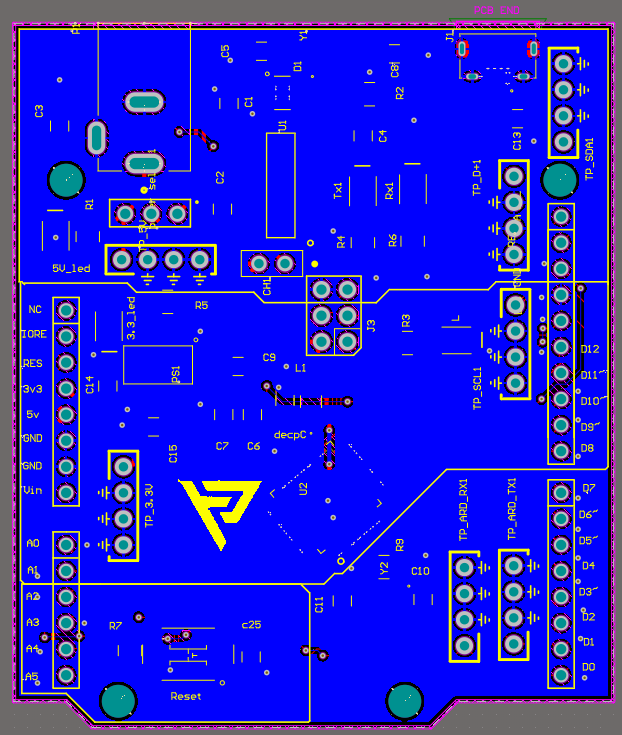
\includegraphics[scale=0.6]{figures/pcb/bottom_layer.png}
	\caption{Bottom layer}
	\label{top}
\end{figure}

\begin{figure}[H]
	\centering
	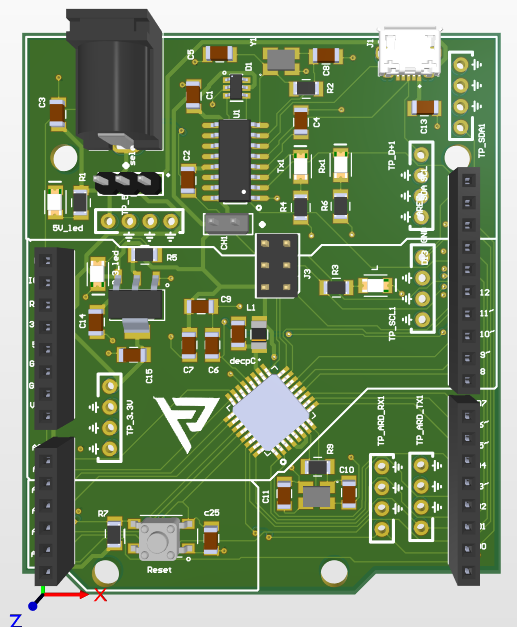
\includegraphics[scale=0.6]{figures/pcb/3d.png}
	\caption{3D view}
	\label{top}
\end{figure}



This is the photo of the PCB after manufacturing\\

\begin{figure}[H]
	\centering
	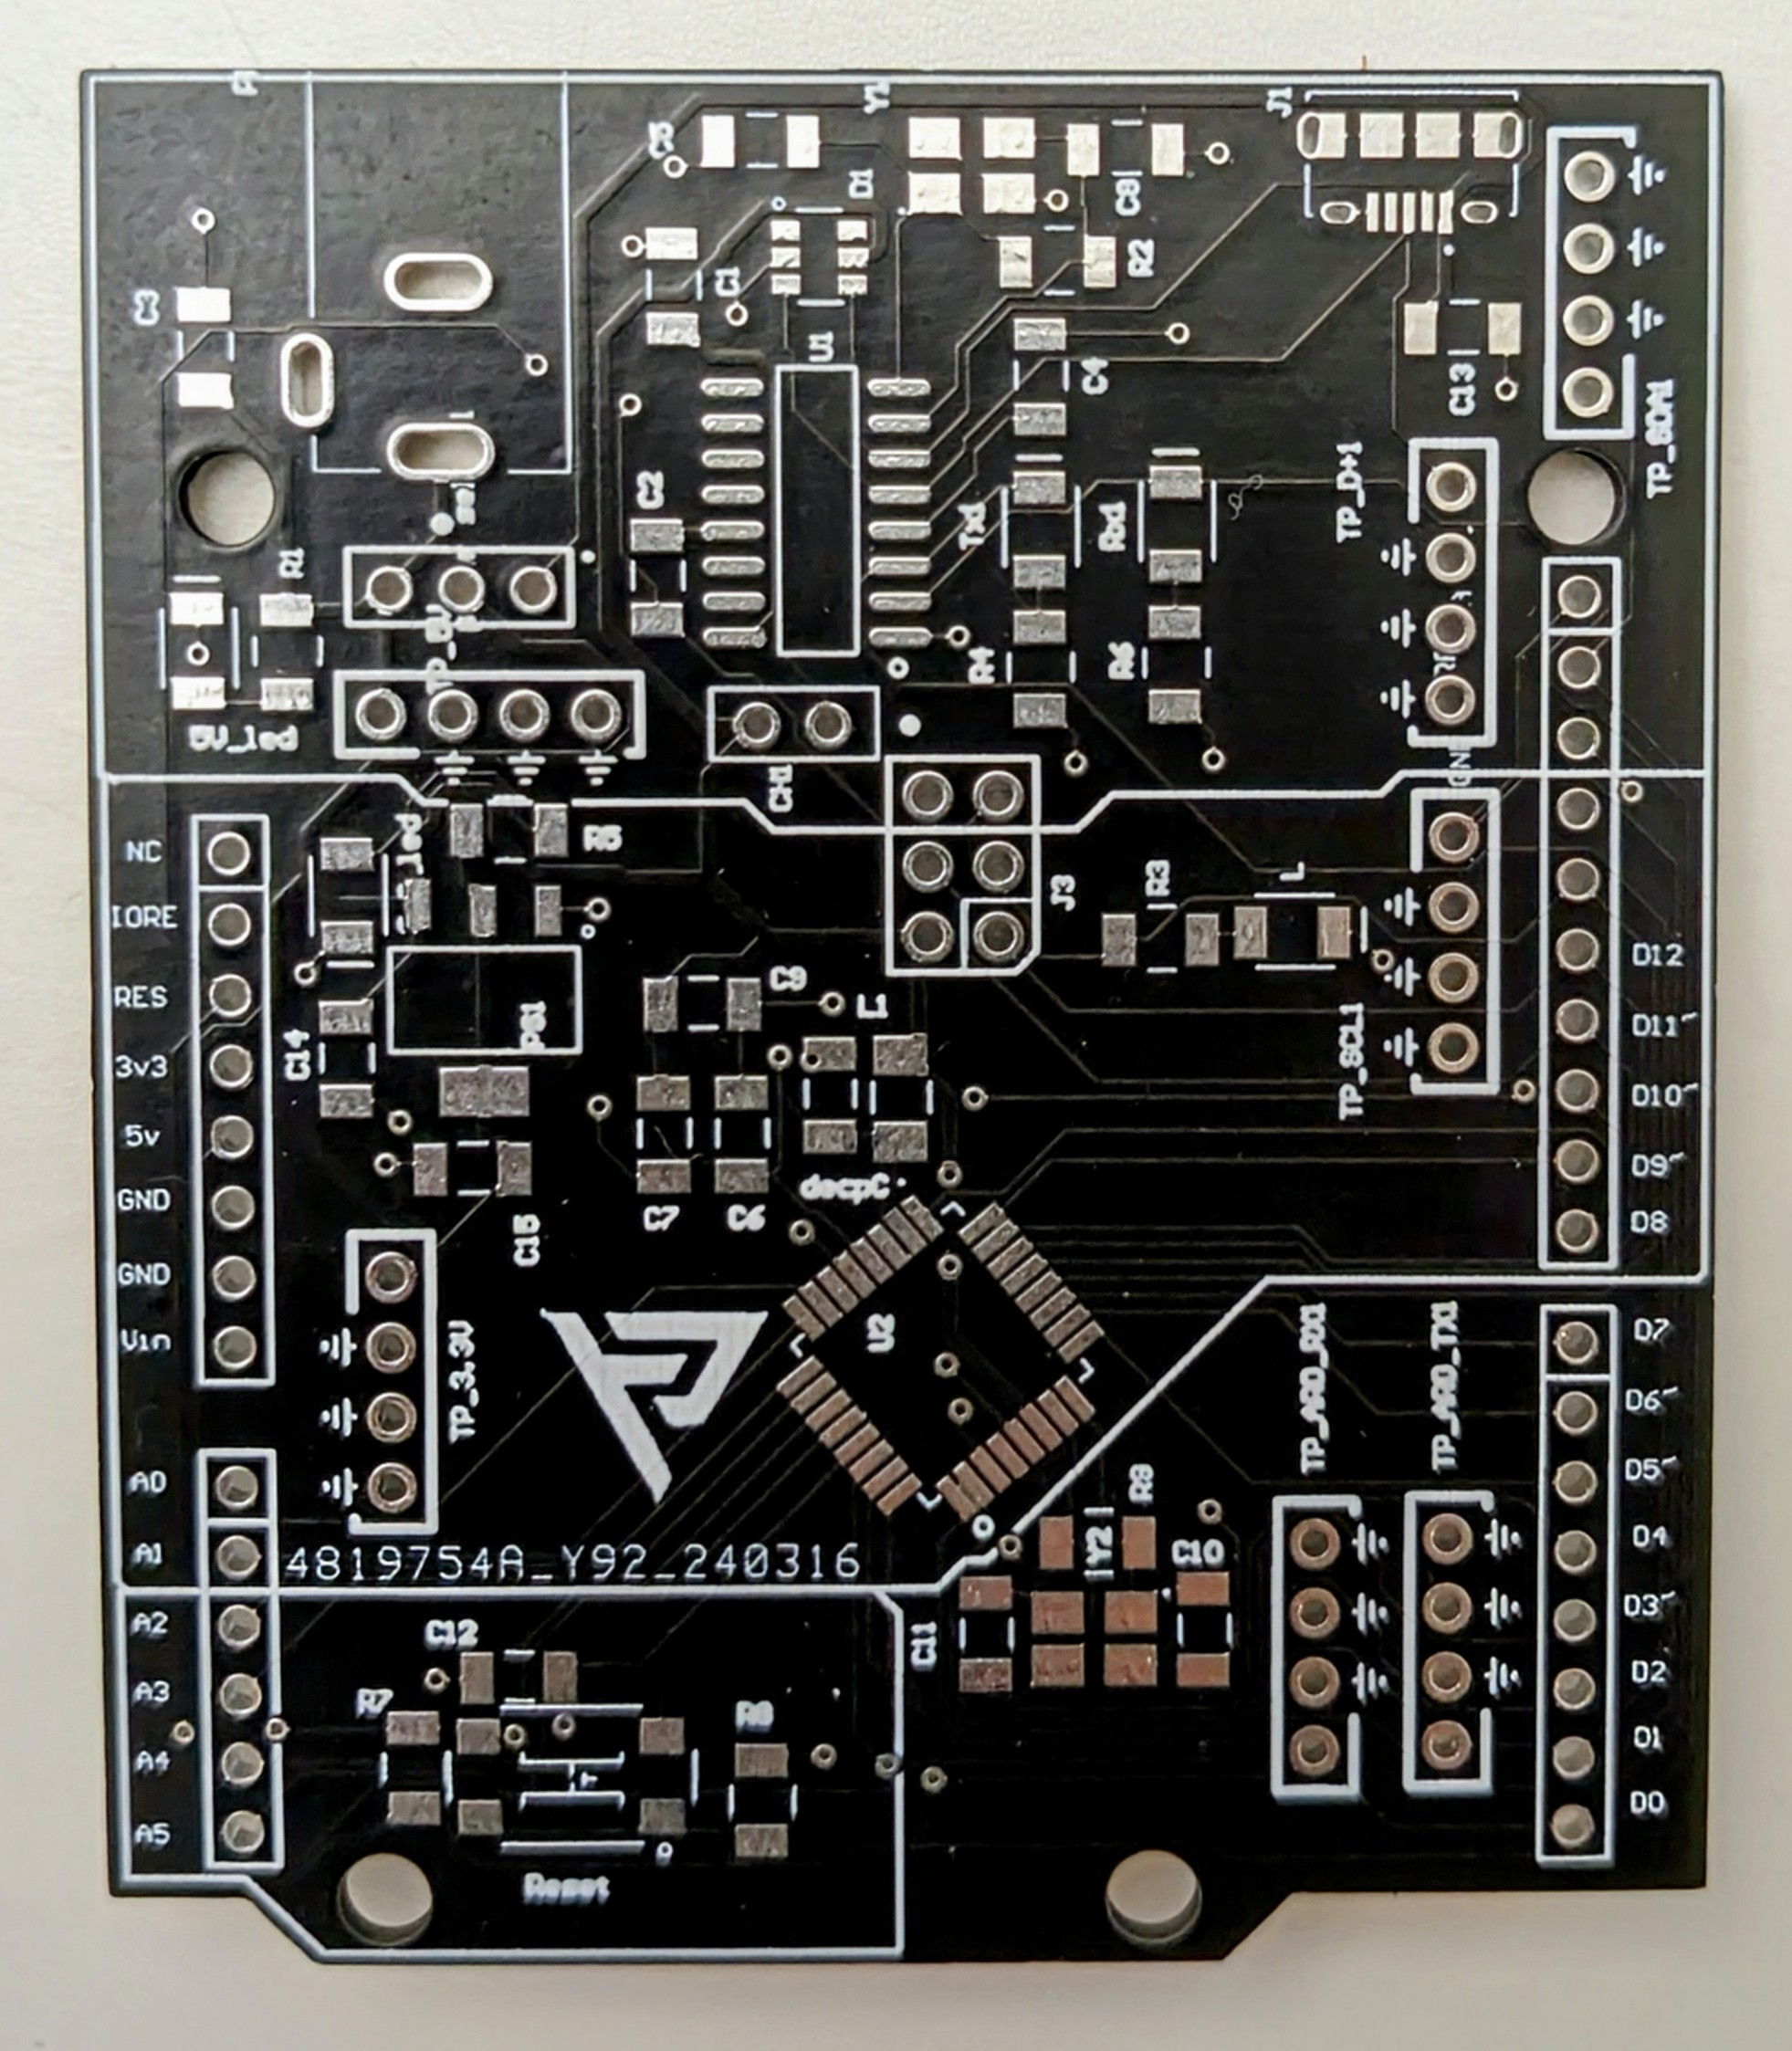
\includegraphics[scale=0.25]{figures/without_component.jpg}
	\caption{Without component}
	\label{top}
\end{figure}

\begin{figure}[H]
	\centering
	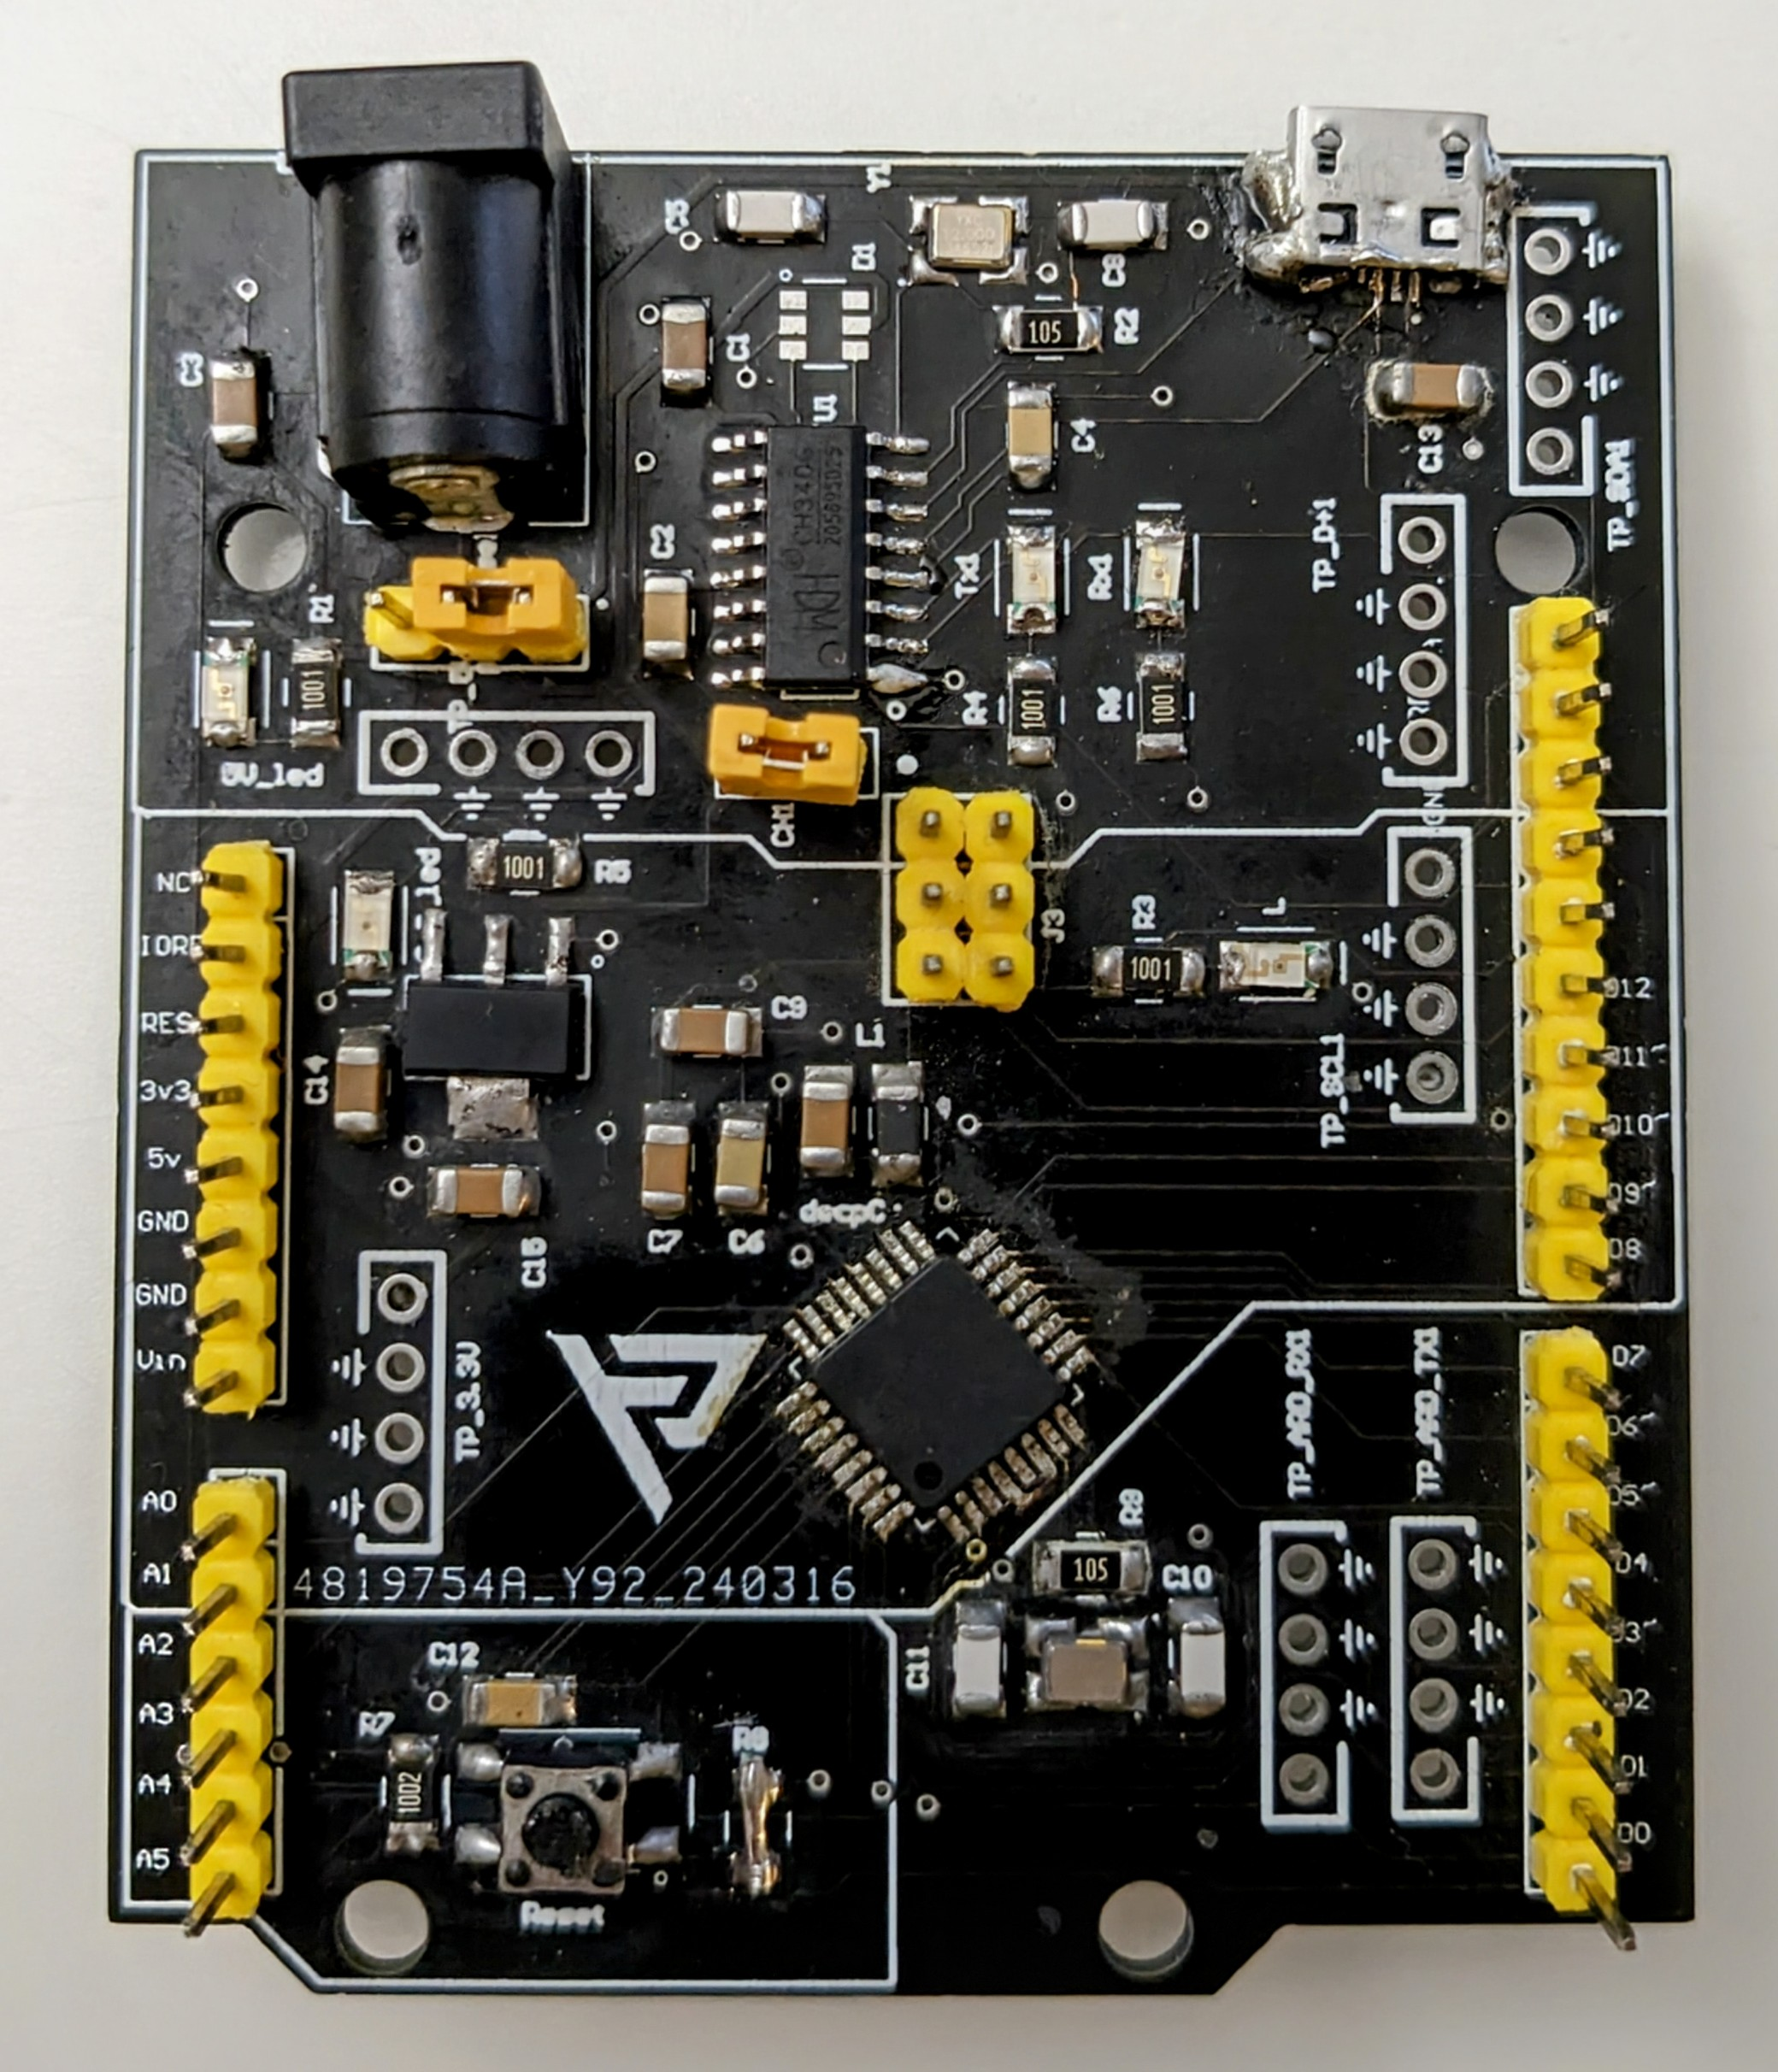
\includegraphics[scale=0.2]{figures/with_component.jpg}
	\caption{With component}
\end{figure}

\begin{figure}[H]
	\centering
	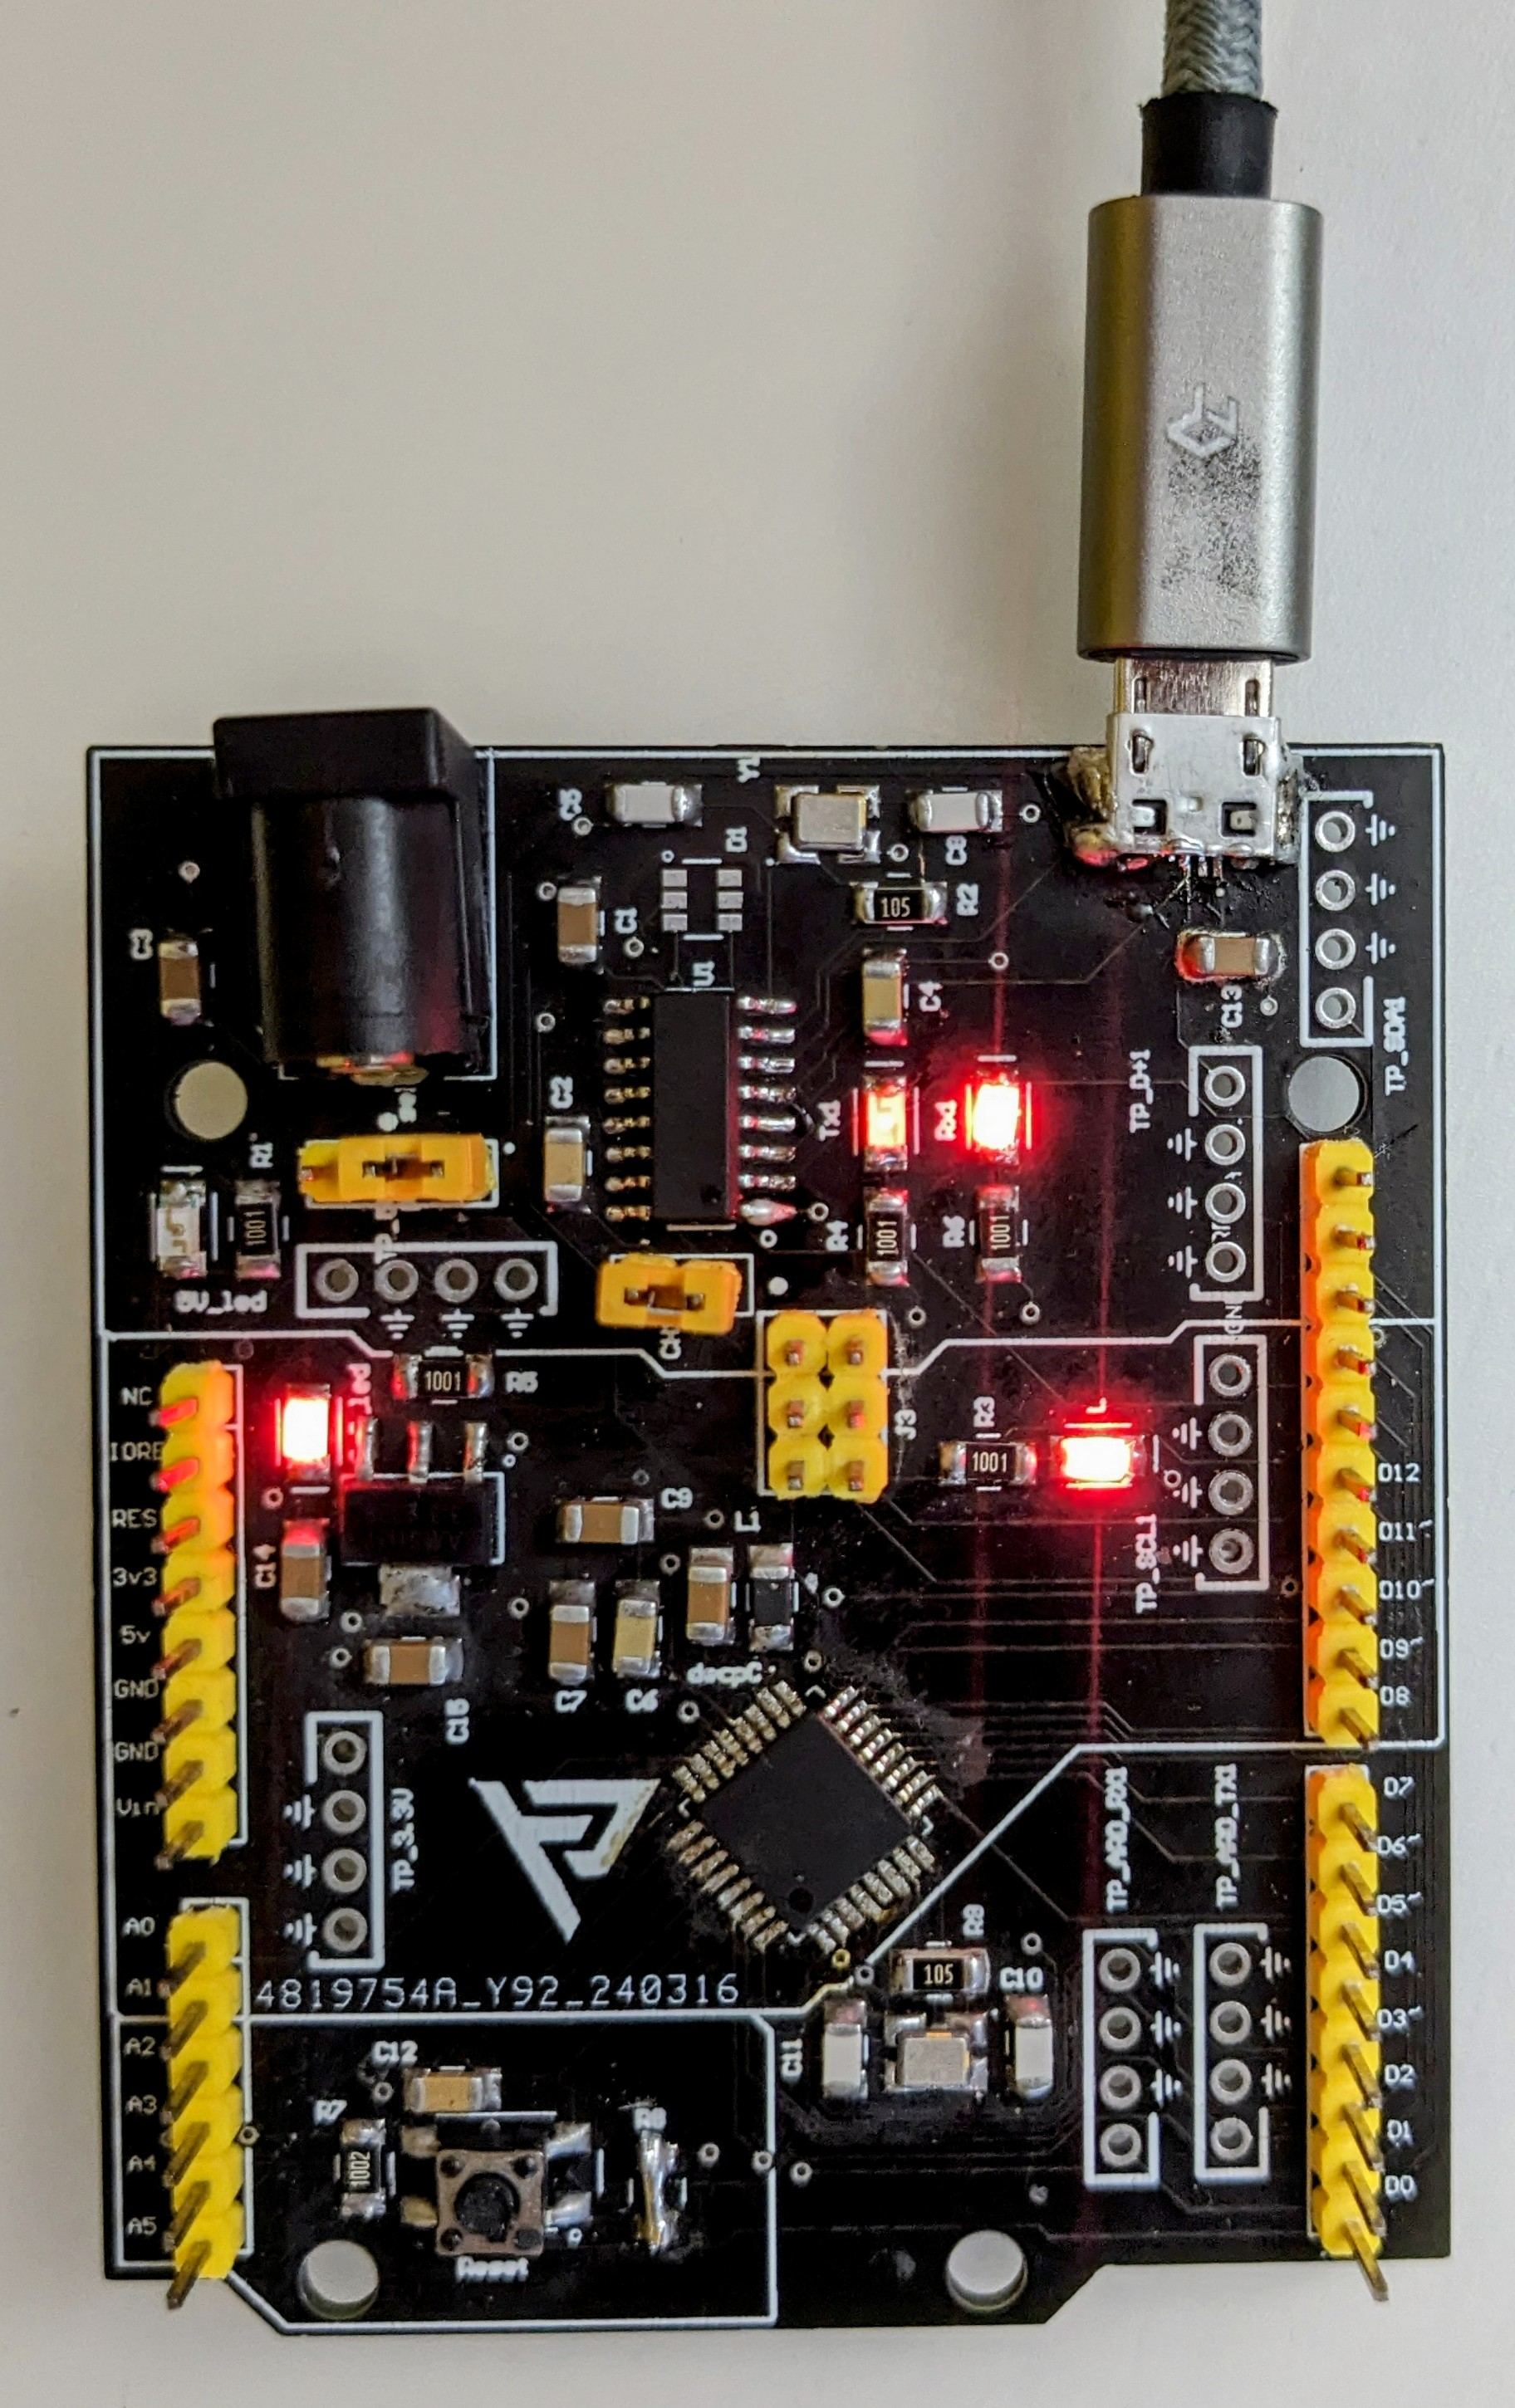
\includegraphics[scale=0.2]{figures/working_board.jpg}
	\caption{First program running}
\end{figure}


\begin{figure}[H]
	\centering
	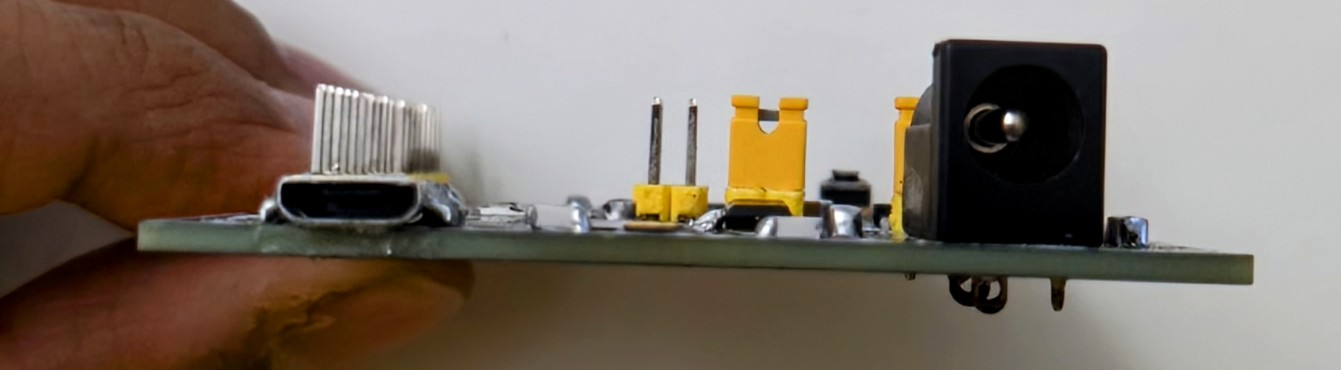
\includegraphics[scale=0.35]{figures/usb.jpg}
	\caption{\textbf{I have used micro b instead of mini B connector}}
\end{figure}


\textbf{Arduino noise Shield}

\begin{figure}[H]
	\centering
	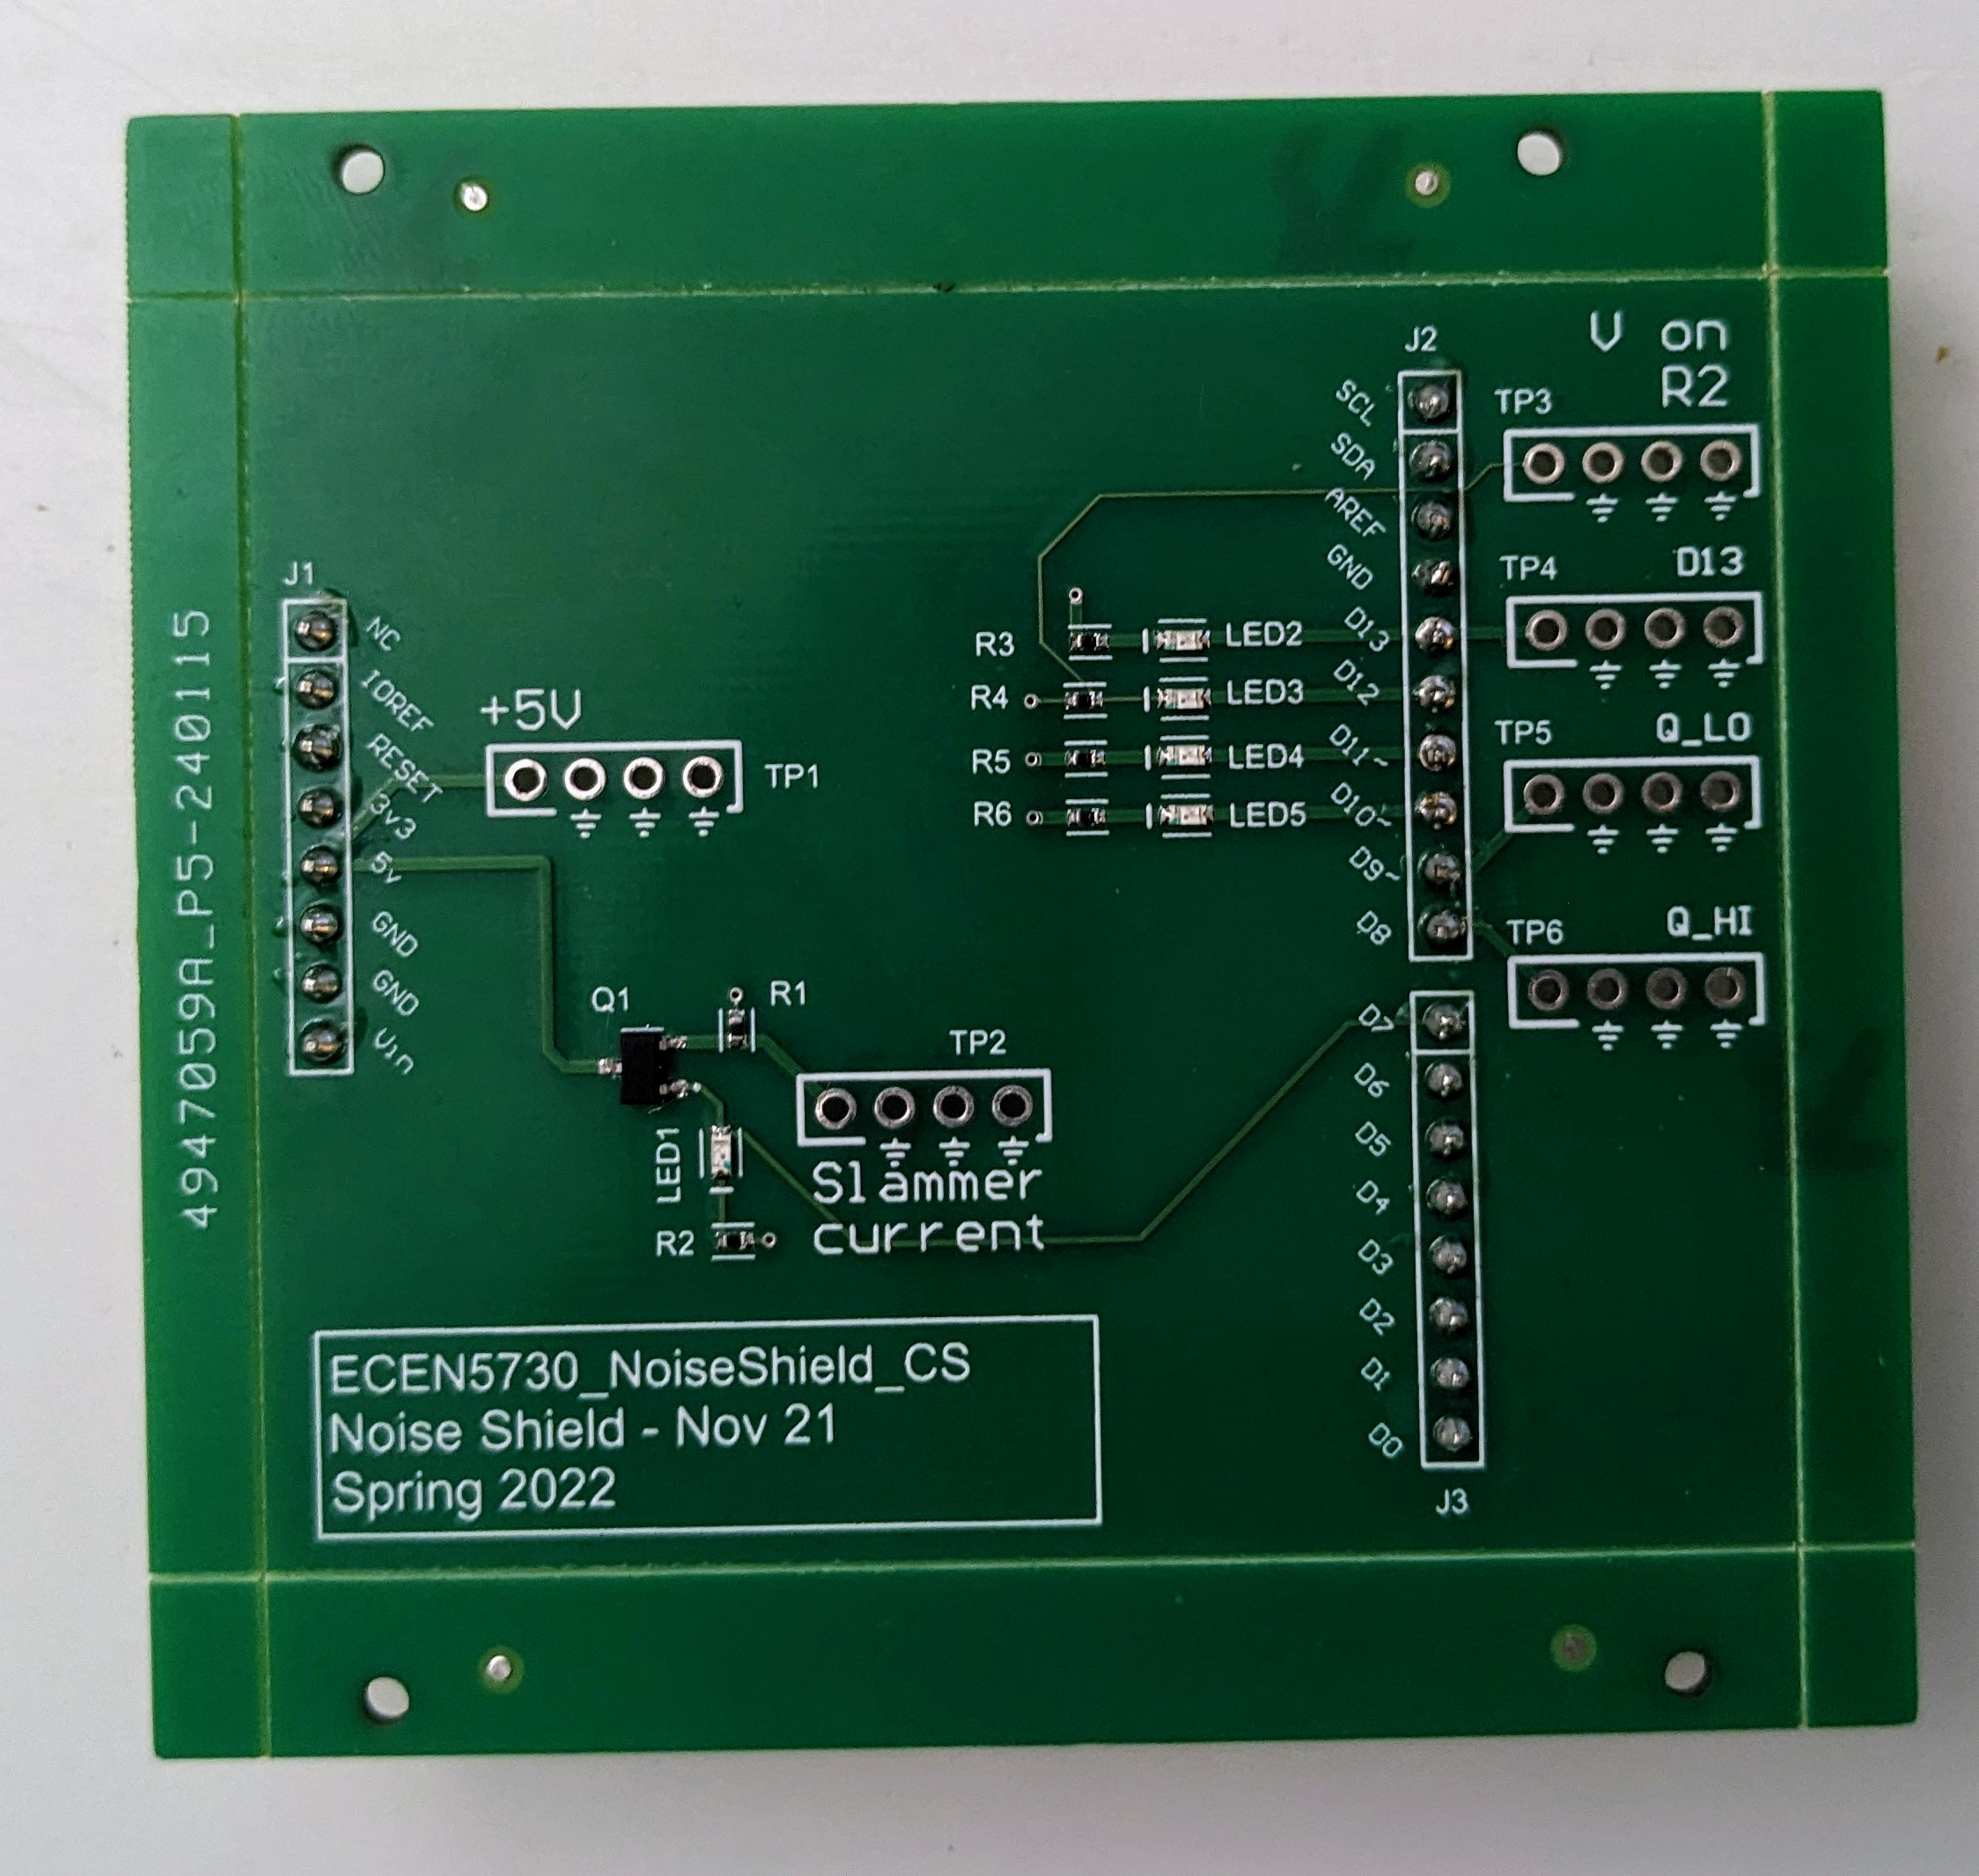
\includegraphics[scale=0.2]{figures/arduino_shield.jpg}
	\caption{Noise Shield used for taking reading}
\end{figure}



below is the details of the power section, Atmega328 microcontroller, test probes, and oscillator sections of the PCB layout, and how they are interconnected based on the schematic.

\begin{enumerate}
	\item Power Section:
	      \begin{itemize}
		      \item In the schematic, the power section includes a barrel jack connector and a USB connector for power input. The PCB layout reflects these components as J3 (barrel jack) and J1 (USB connector).
		      \item The power from the barrel jack and USB connector is routed to the voltage regulator (U1) on the PCB. The voltage regulator is responsible for converting the input voltage to a stable 3.3V supply for the microcontroller and other components.
		      \item On the PCB, the power traces from the input connectors to the voltage regulator are typically wider to handle higher currents and reduce voltage drops. The output of the voltage regulator is then distributed to the microcontroller and other parts of the circuit through power traces.
		      \item The schematic also includes decoupling capacitors near the power input and voltage regulator to filter out noise and stabilize the power supply. These capacitors are placed close to the respective components on the PCB layout to minimize trace lengths and improve power stability.
	      \end{itemize}



	\item Atmega328 Microcontroller:
	      \begin{itemize}
		      \item The Atmega328 microcontroller (U2) is the central component of the Arduino clone. In the schematic, the microcontroller is shown with its various pin connections.

		      \item On the PCB layout, the Atmega328 is positioned strategically to minimize trace lengths and facilitate easy routing of signals. The power pins (VCC and GND) of the microcontroller are connected to the regulated 3.3V supply and ground, respectively, through the power traces.

		      \item The other pins of the microcontroller, such as the digital I/O pins, analog input pins, and communication pins (e.g., UART, SPI, I2C), are routed to their respective headers or connectors on the PCB. The trace lengths are kept as short as possible to minimize signal integrity issues and reduce noise.

		      \item The ICSP header (J2) is connected to the appropriate pins of the Atmega328 to enable in-circuit programming and debugging. The traces for the ICSP signals (MISO, MOSI, SCK, and RESET) are routed carefully to ensure reliable programming and communication.
	      \end{itemize}

	\item Crystal Oscillators:
	      There are two crystal oscillators located near the microcontroller, labeled as "Y1" (16MHz) and "Y2" (12MHz).\\
	      The proximity of the oscillators to the microcontroller minimizes trace lengths and ensures stable clock signals.
	\item Voltage Regulator:
	      The voltage regulator, likely a 3.3V LDO (Low Dropout), is labeled as "U1".
	      The regulator is positioned close to the power input and has input and output feedback capacitor to stable the output (reduce ringing)
	\item USB Interface:
	      The USB interface is located on the left side of the board, labeled as "J1".
	\item Power Input:
	      The power input section includes a barrel jack connector (J3) and a USB connector (J1), providing options for powering the board.
	\item ICSP Header:\textbf{(There is an error in the ICSP routing/ Hard error)}
	      The ICSP (In-Circuit Serial Programming) header is labeled as "J2".\\
	      The ICSP header allows for direct programming of the microcontroller using an external programmer.
	\item Headers and Connectors:
	      The layout includes several headers and connectors for interfacing with external devices and peripherals.\\
	      These include headers for power (J4, J5), analog inputs (J6), and digital inputs/outputs (J7, J8).
	\item Ground Plane:
	      The PCB layout incorporates a solid ground plane, which helps to reduce noise, improve signal integrity, and provide a low-impedance return path for currents.
\end{enumerate}




\section{Code / Bootloading }
Connect ARDUINO pins to new Atmega328P for bootloading
here is the wiring diagram
\begin{figure}[H]
	\centering
	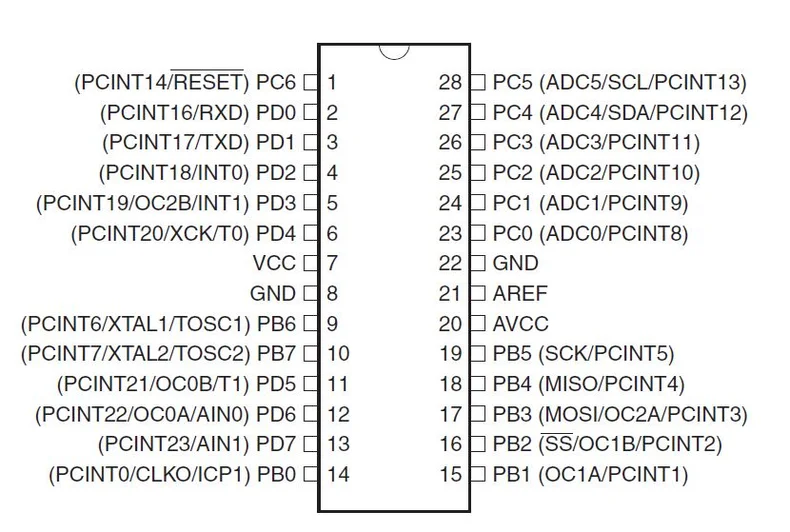
\includegraphics[scale=0.6]{figures/bootload1.png}
	\caption{First time turning on the PCB and selecting good layout}
\end{figure}

UNO 5v ---> ATmega pin 7 (VCC)\\
UNO GND ---> ATmega pin 8 (GND)\\
UNO pin 10 ---> ATmega pin 1 (RESET)\\
UNO pin 11 ---> ATmega pin 17 (MOSI)\\
UNO pin 12 ---> ATmega pin 18 (MISO)\\
UNO pin 13 ---> ATmega pin 19 (SCK)\\

\begin{enumerate}
	\item Each microprocessor has a signature – a unique code that identifies its model. When you bootload a chip (or even upload a sketch) the Arduino IDE checks that the chip selected matches the type it’s connected to. Even though the ATmega328-PU in essence functions in the same way as the ATmega328P-PU, it has a different signature, and one that isn’t recognised by the Arduino IDE.
	\item If we try to bootload an ATmega328-PU, we get a message something along the lines of:\\
	      avrdude: Device signature = 0x1e9514\\
	      avrdude: Expected signature for ATMEGA328P is 1E 95 0F\\
	      Double check chip, or use -F to override this check.\\
	      \begin{figure}[H]
		      \centering
		      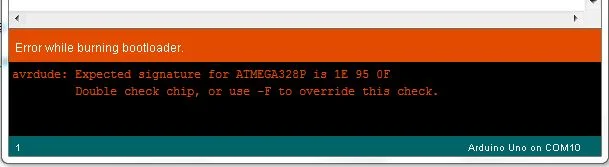
\includegraphics[scale=0.6]{figures/bootload_error.png}
		      \caption{First time turning on the PCB and selecting good layout}
	      \end{figure}

	\item The way to work around this is to “trick” the IDE into believing your 328-PU is in fact a 328P-PU. Disclaimer: I have tested this myself and it works.\\
	      \begin{itemize}
		      \item Make a backup copy of the file: avrdude.conf
		      \item Open the file avrdude.conf in a text editor
		      \item Search for: “0x1e 0x95 0x0F” (this is the ATmega328P signature)
		      \item Replace it with: “0x1e 0x95 0x14” (this is the ATmega328 signature)
		      \item Save the file
		      \item Restart the Arduino IDE
		      \item Once bootloading is complete restore the backup copy you made.
	      \end{itemize}
	\item Bootload the ATmega328:\\
	      In the Arduino IDE, from the Tools menu:
	      \begin{itemize}
		      \item under the Board option choose Arduino UNO
		      \item under the Serial Port option ensure the correct port is selected
		      \item under the Programmer option choose Arduino as ISP
		      \item To burn the Bootloader, choose Burn Bootloader from the Tools menu
		      \item we should see a message “Burning bootloader to I/O Board (this may take a minute)"
	      \end{itemize}

	\item Once the bootloader has been burned, you’ll see a message confirming the success. and now we can upload the code directly to golden Arduino
	\item Upload following code
	      \begin{lstlisting}
// the setup function runs once when you press reset or power the board
void setup() {
  // initialize digital pin LED\_BUILTIN as an output.
  pinMode(LED\_BUILTIN, OUTPUT);
}

// the loop function runs over and over again forever
void loop() {
  digitalWrite(LED\_BUILTIN, HIGH);  // turn the LED on (HIGH is the voltage level)
  delay(1000);                      // wait for a second
  digitalWrite(LED\_BUILTIN, LOW);   // turn the LED off by making the voltage LOW
  delay(1000);                      // wait for a second
}
\end{lstlisting}


\end{enumerate}


\textbf{Code for Noise shield}

\begin{lstlisting}
void setup() {
	DDRB = B00111111;
	pinMode(7, OUTPUT);
	digitalWrite(7, LOW);
}
void loop() {
	PORTB = B00111101;
	delayMicroseconds(4);
	PORTB = B00000001;
	delay(1);
	digitalWrite(7, HIGH);
	delayMicroseconds(400);
	digitalWrite(7, LOW);
	delay(10);
}
	\end{lstlisting}





\textit{Source from instructables.com}


\section{Output Waveforms / Measurement}
\begin{enumerate}
	\item Output at D13 pin ! (blinky program)
	      \begin{figure}[H]
		      \centering
		      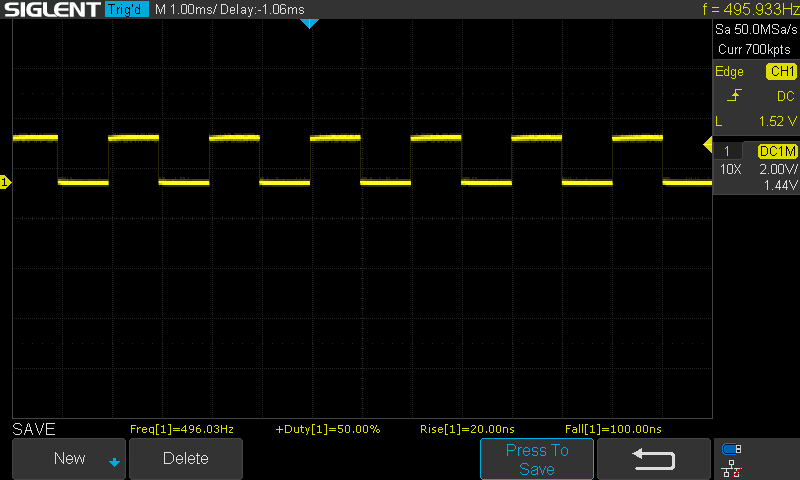
\includegraphics[scale=0.6]{figures/output.png}
		      \caption{Blinky Program output}
	      \end{figure}
	\item Current through 47ohm resistor
	      \begin{itemize}

		      \item Golden Arduino:
		            \begin{figure}[H]
			            \centering
			            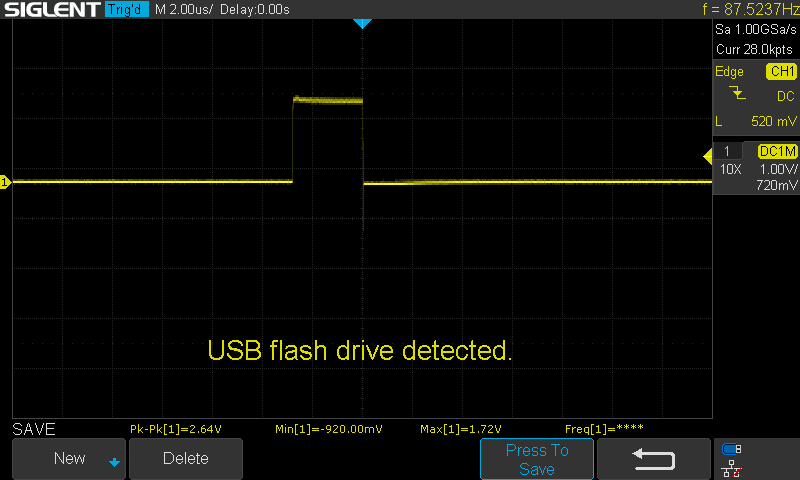
\includegraphics[scale=0.6]{figures/drop.png}
			            \caption{Drop of 47 ohm in the shield}
		            \end{figure}
		            The screenshot above depicts the voltage drop across a 47-ohm resistor connected to the Golden Arduino board. The measured voltage drop is approximately 2.5 volts. Applying Ohm's law, the current through the resistor can be determined as:


		            \begin{flalign*}
			             & I = \frac{V}{R}    &  & \\\\
			             & I = \frac{2.5}{63} &  & \\
			             & I = 53.191489 mA   &  & \\\\
		            \end{flalign*}

	      \end{itemize}

	\item Switching noise on Quiet Low pin and Power rail
	      \begin{itemize}
		      \item Commercial Arduino:
		            \begin{figure}[H]
			            \centering
			            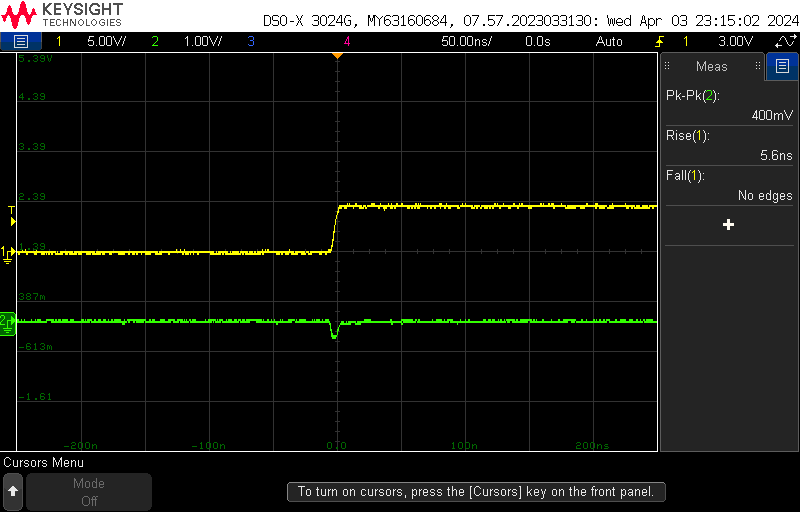
\includegraphics[scale=0.6]{figures/commercial_ard/d13_trig_ql.png}
			            \caption{switching noise on quiet low pin for rising edge}
		            \end{figure}

		            \begin{figure}[H]
			            \centering
			            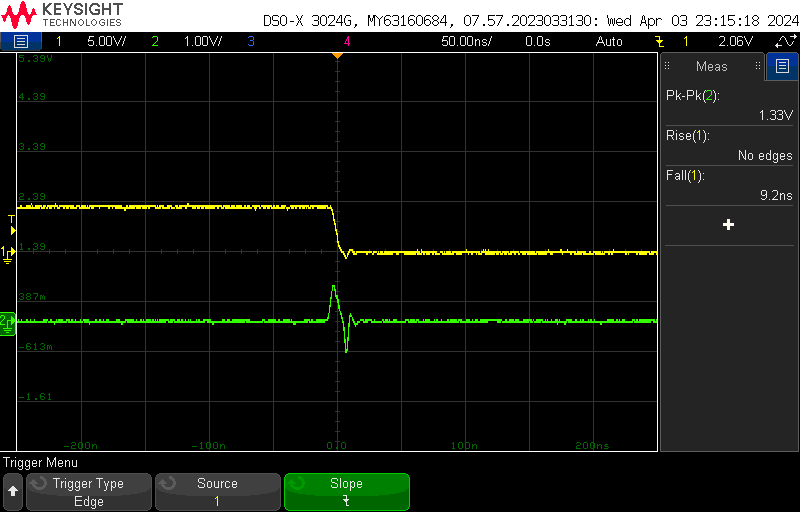
\includegraphics[scale=0.6]{figures/commercial_ard/d13_trig_ql_fall.png}
			            \caption{switching noise on quiet low pin for falling edge}
		            \end{figure}

		            \begin{figure}[H]
			            \centering
			            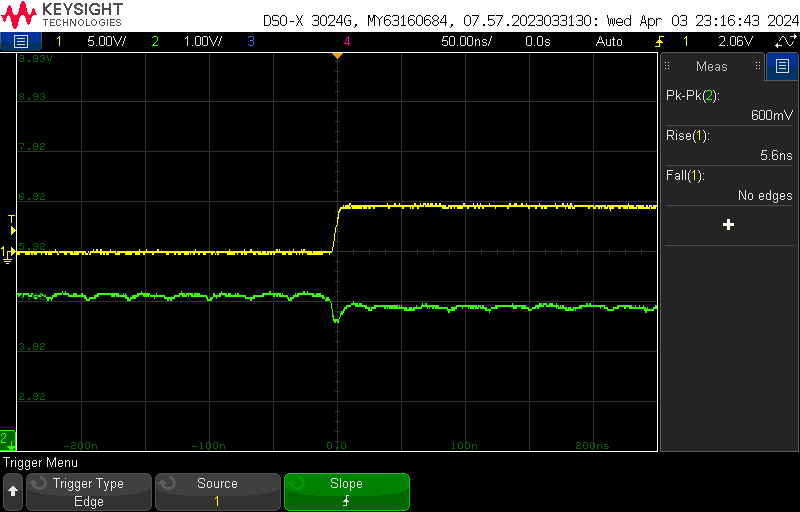
\includegraphics[scale=0.6]{figures/commercial_ard/d13_trig_qh_rise.png}
			            \caption{switching noise on quiet high pin for rising edge}
		            \end{figure}

		            

					\begin{figure}[H]
			            \centering
			            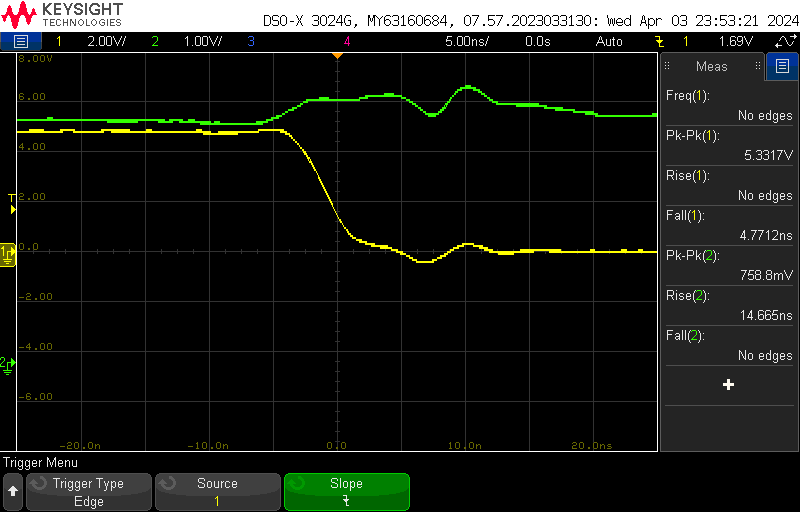
\includegraphics[scale=0.6]{figures/my_ard/d13_trig_qh_fall.png}
			            \caption{switching noise on quiet high pin for falling edge}
		            \end{figure}

		            The above screenshots illustrate the switching noise observed on the quiet low pin and 5V power rail of the commercial Arduino board. The yellow trace represents the trigger signal (switching pin D13), while the green trace shows the noise signal captured on the respective pin or power rail.
		      \item Golden Arduino:

		            \begin{figure}[H]
			            \centering
			            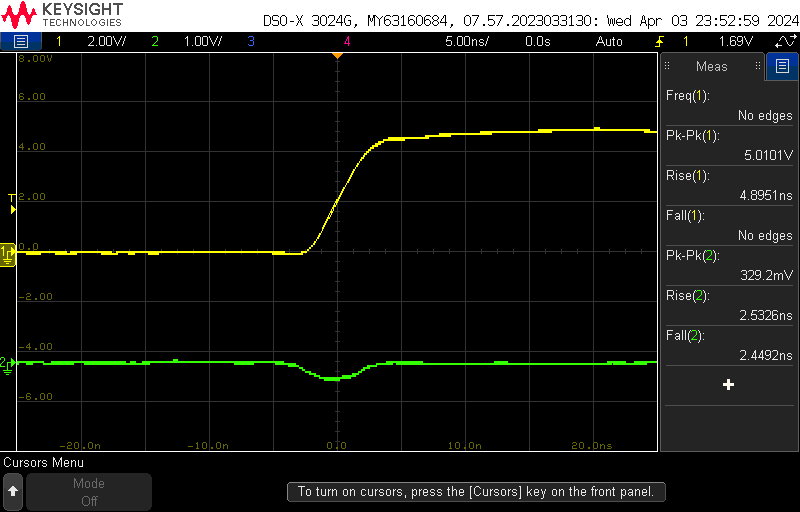
\includegraphics[scale=0.6]{figures/my_ard/d13_trig_ql_rise.png}
			            \caption{switching noise on quiet low pin for rising edge}
		            \end{figure}

		            \begin{figure}[H]
			            \centering
			            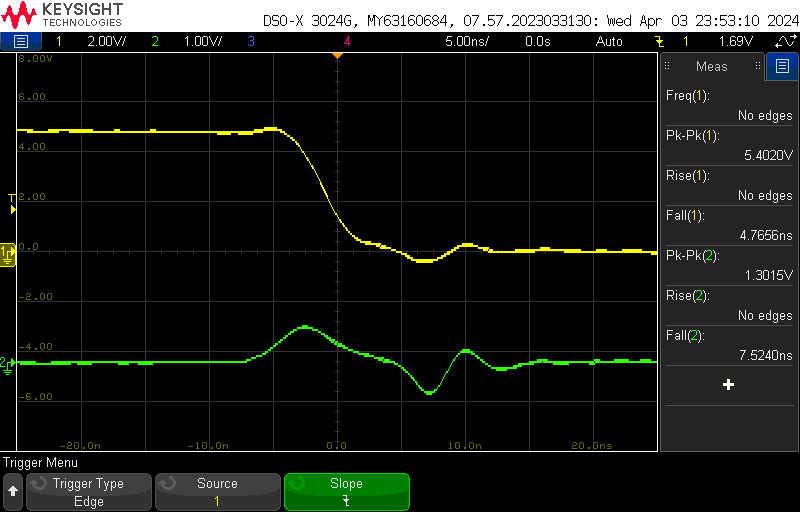
\includegraphics[scale=0.6]{figures/my_ard/d13_trig_ql_fall.png}
			            \caption{switching noise on quiet low pin for falling edge}
		            \end{figure}

		            \begin{figure}[H]
			            \centering
			            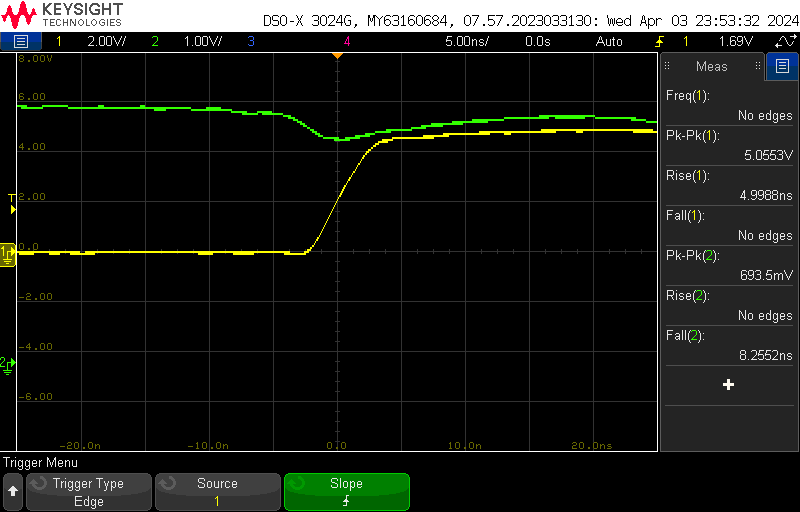
\includegraphics[scale=0.6]{figures/my_ard/d13_trig_qh_rise.png}
			            \caption{switching noise on quiet high pin for rising edge}
		            \end{figure}

					\begin{figure}[H]
			            \centering
			            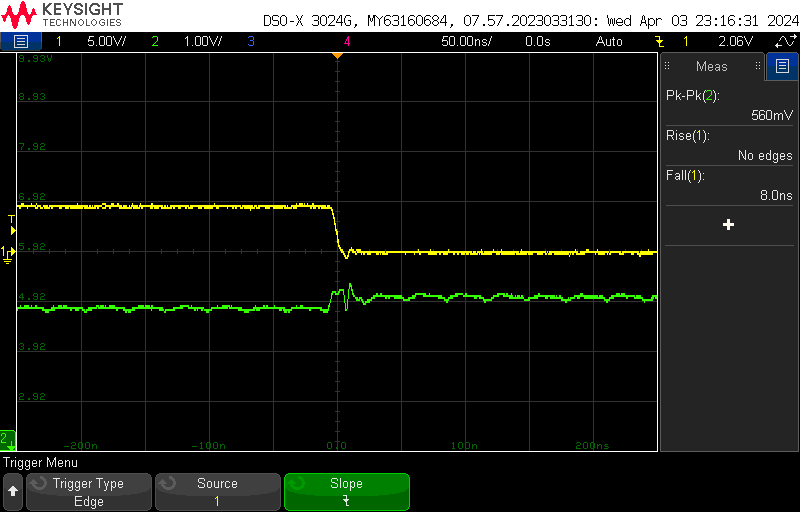
\includegraphics[scale=0.6]{figures/commercial_ard/d13_trig_qh_fall.png}
			            \caption{switching noise on quiet high pin for falling edge}
		            \end{figure}
		            

		            Similar to the commercial Arduino, the screenshots above demonstrate the switching noise observed on the quiet low pin and 5V power rail of the Golden Arduino board. The yellow trace indicates the trigger signal (switching pin D13), and the green trace represents the noise signal captured on the corresponding pin or power rail.
	      \end{itemize}

		  \begin{table}[H]
			\centering
			\begin{tabular}{ |l |c | c|}
				\hline
				\textbf{Layout}                                            & \textbf{Quite High Noise} & \textbf{Quite Low Noise} \\\hline
																		   &                           &                          \\
				Commercial                                                &
				\begin{tabular}{@{}cc@{}} % Inner table with two columns
					\textbf{Rise} & \textbf{Fall} \\
					600 mV       & 760 mV         \\
				\end{tabular} &
				\begin{tabular}{@{}cc@{}} % Inner table with two columns
					\textbf{Rise} & \textbf{Fall} \\
					400mV         & 1.33 V         \\
				\end{tabular}                                                         \\
		
				Golden Arduino                                                 &
				\begin{tabular}{@{}cc@{}} % Inner table with two columns
					600 mV & 580 mV \\
				\end{tabular} &
				\begin{tabular}{@{}cc@{}} % Inner table with two columns
					329mV & 1 V \\
				\end{tabular}                                                         \\
		
				\hline\hline
			\end{tabular}
			\caption{Noise Measurement}
			\label{filterspecs}
		\end{table}
		
		
		The table above compares the switching noise levels measured on the commercial Arduino and Golden Arduino boards. It can be observed that the Golden Arduino exhibits lower noise levels compared to the commercial Arduino. This improvement can be attributed to factors such as better component placement, proper decoupling techniques, and optimized PCB layout in the Golden Arduino design.

	\item Noise on Power rail when board is aggressor
	      \begin{itemize}
		      \item Commercial Arduino:
		      \begin{figure}[H]
				\centering
				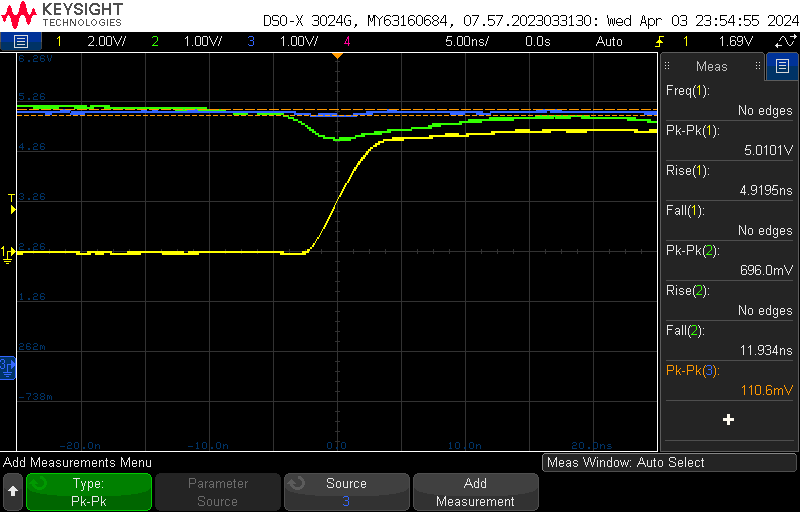
\includegraphics[scale=0.6]{{figures/my_ard/d13_trig_power_qh.png}}
				\caption{switching noise on 5V power rail for rising edge}
			\end{figure}

			\begin{figure}[H]
				\centering
				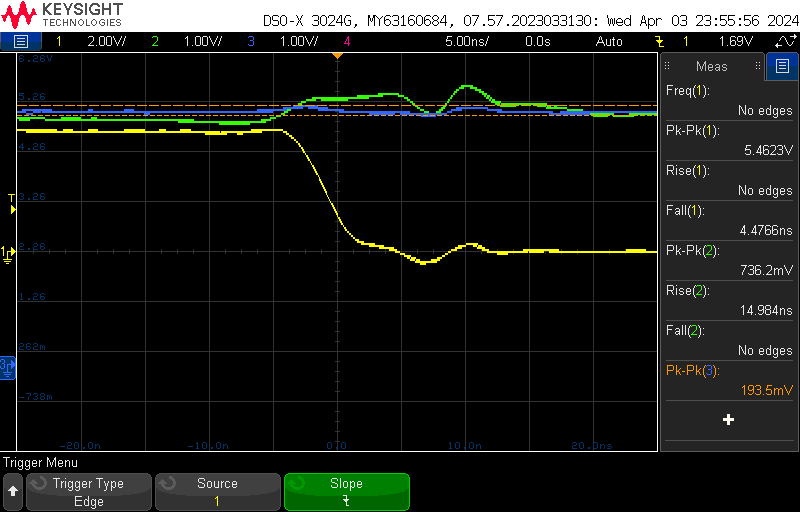
\includegraphics[scale=0.6]{figures/my_ard/power_qh_fall.png}
				\caption{switching noise on 5V power rail for falling edge}
			\end{figure}
		           

		      \item Golden Arduino:
			  \begin{figure}[H]
				\centering
				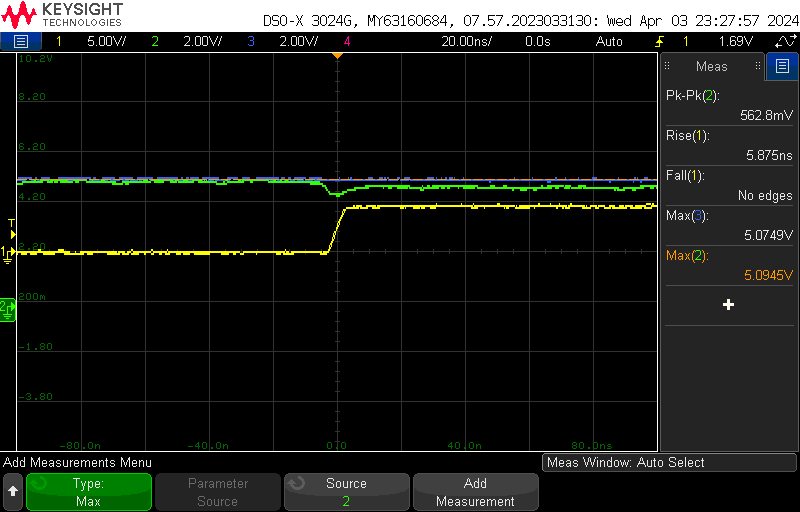
\includegraphics[scale=0.6]{{figures/commercial_ard/power_qh_rising.png}}
				\caption{switching noise on 5V power rail for rising edge}
			\end{figure}

			\begin{figure}[H]
				\centering
				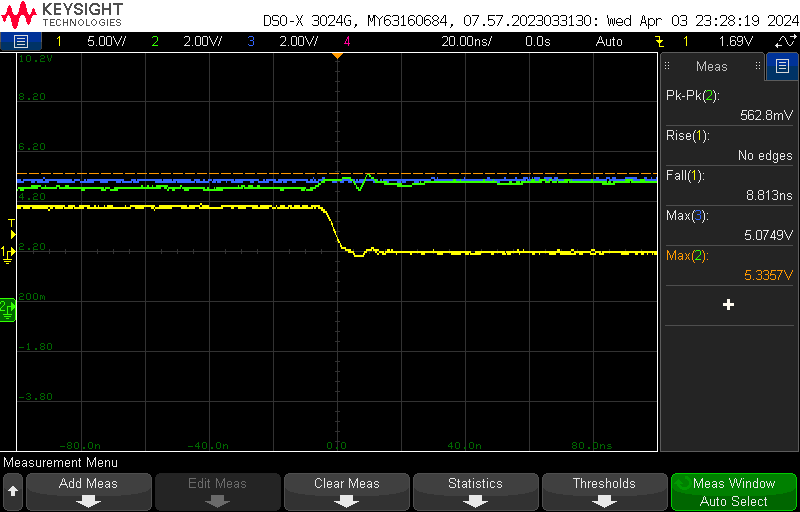
\includegraphics[scale=0.6]{figures/commercial_ard/power_qh_falling.png}
				\caption{switching noise on 5V power rail for falling edge}
			\end{figure}


		      \item The screenshots above show the noise observed on the power rail when the respective Arduino board itself acts as an aggressor, generating noise through switching activity. The yellow trace represents the trigger signal, while the green trace captures the noise on the power rail.
			           
\begin{table}[H]
	\centering
	\begin{tabular}{ |l |c | c|}
		\hline
		\textbf{Layout}                                            & \textbf{Noise}  \\\hline
		                                                           &                                                   \\
		Commercial                                                &
		\begin{tabular}{@{}cc@{}} % Inner table with two columns
			\textbf{Rise} & \textbf{Fall} \\
			600 mV       & 700 mV         \\
		\end{tabular}                                                       \\

		Golden arduino                                                 &
		\begin{tabular}{@{}cc@{}} % Inner table with two columns
			562 mV & 562 mV \\
		\end{tabular}                                                        \\

		\hline\hline
	\end{tabular}
	\caption{Noise Measurement}
	\label{filterspecs}
\end{table}
		            The table compares the noise levels on the power rail when the commercial Arduino and Golden Arduino boards are acting as aggressors. It is evident that the Golden Arduino demonstrates improved noise performance, with lower noise levels compared to the commercial Arduino. This enhancement can be attributed to the optimized PCB layout, proper grounding, and effective decoupling techniques employed in the Golden Arduino design.
	      \end{itemize}
	\item Noise on Power rail in slammer circuit
	      \begin{itemize}
		      \item Commercial Arduino:
		            \begin{figure}[H]
			            \centering
			            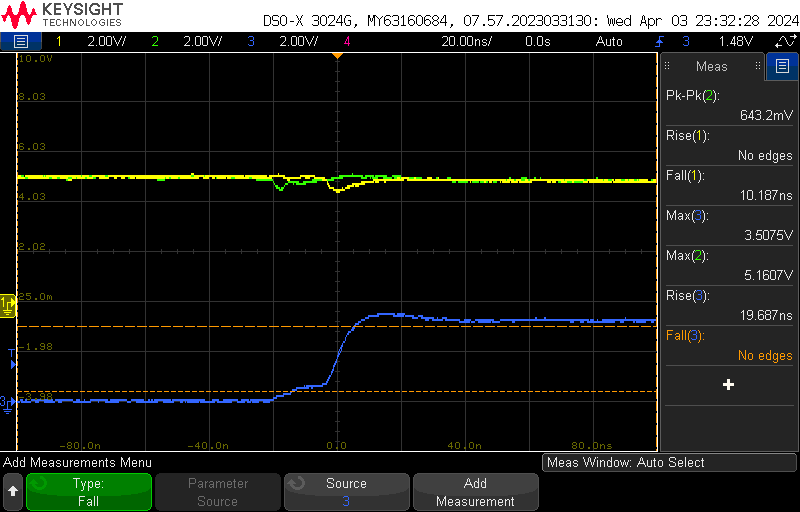
\includegraphics[scale=0.6]{{figures/commercial_ard/rising_slammer.png}}
			            \caption{switching noise on 5V power rail for rising edge}
		            \end{figure}

		            \begin{figure}[H]
			            \centering
			            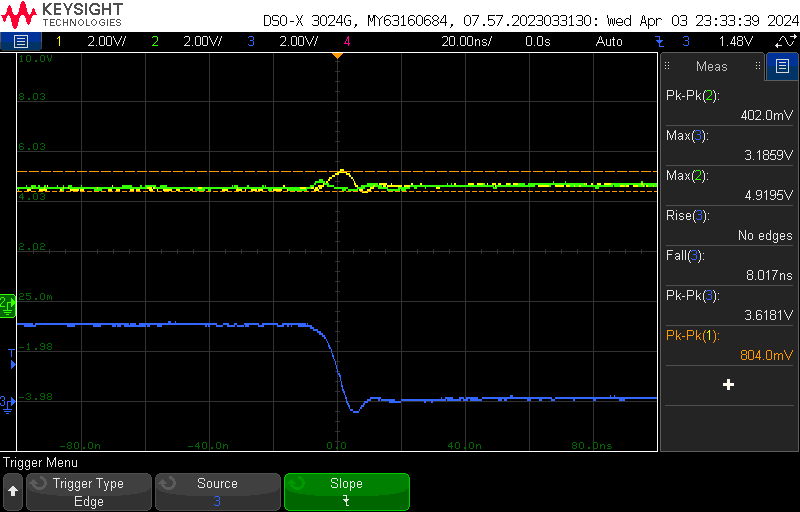
\includegraphics[scale=0.6]{figures/commercial_ard/falling_slammer.png}
			            \caption{switching noise on 5V power rail for falling edge}
		            \end{figure}

		      \item Golden Arduino:
		            \begin{figure}[H]
			            \centering
			            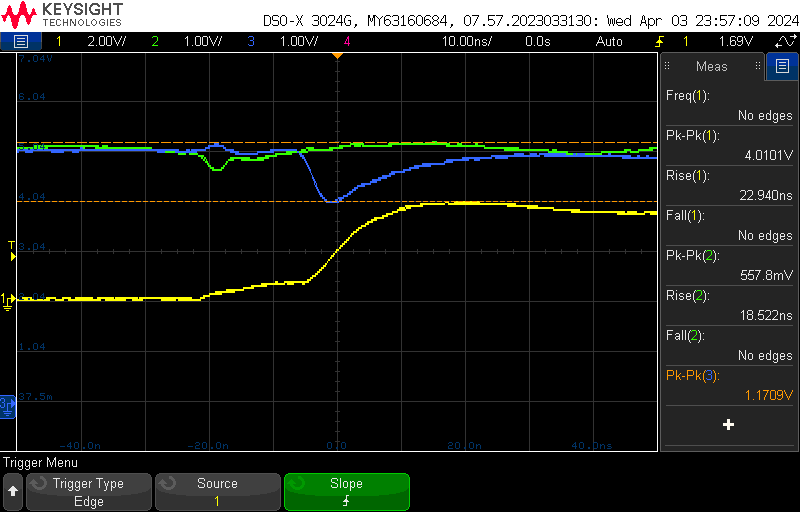
\includegraphics[scale=0.6]{{figures/my_ard/slammer_rise.png}}
			            \caption{switching noise on 5V power rail for rising edge}
		            \end{figure}

		            \begin{figure}[H]
			            \centering
			            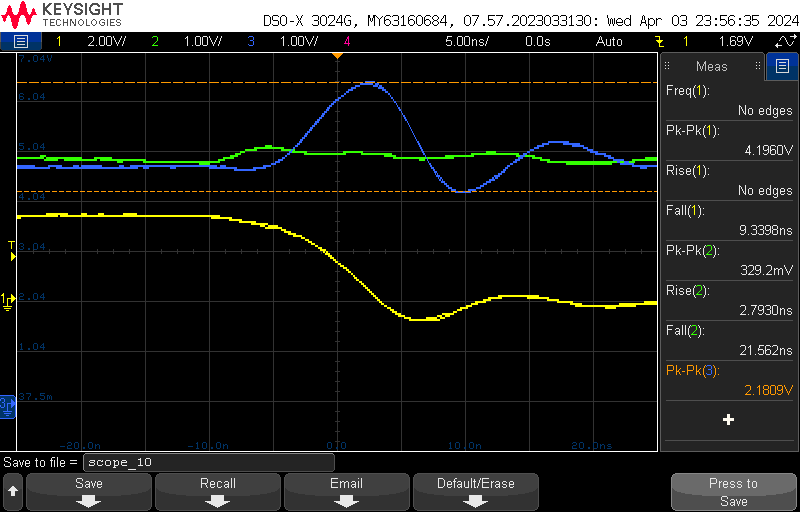
\includegraphics[scale=0.6]{figures/my_ard/slammer_fall.png}
			            \caption{switching noise on 5V power rail for falling edge}
		            \end{figure}

		            The screenshots above show the noise observed on the power rail when the respective Arduino board itself acts as an aggressor, generating noise through switching activity. The yellow trace represents the trigger signal, while the green trace captures the noise on the power rail.
			        

\begin{table}[H]
	\centering
	\begin{tabular}{ |l |c | c|}
		\hline
		\textbf{Layout}                                            & \textbf{Slammer output}  \\\hline
		                                                           &                                                  \\
		Good Layout                                                &
		\begin{tabular}{@{}cc@{}} % Inner table with two columns
			\textbf{Rise} & \textbf{Fall} \\
			643 mV       & 402 mV         \\
		\end{tabular}                                                      \\

		Bad Layout                                                 &
		\begin{tabular}{@{}cc@{}} % Inner table with two columns
			557 mV & 329 mV \\
		\end{tabular}                                                      \\

		\hline\hline
	\end{tabular}
	\caption{Noise Measurement}
	\label{filterspecs}
\end{table}

		            The table compares the noise levels on the power rail when the commercial Arduino and Golden Arduino boards are acting as aggressors. It is evident that the Golden Arduino demonstrates improved noise performance, with lower noise levels compared to the commercial Arduino. This enhancement can be attributed to the optimized PCB layout, proper grounding, and effective decoupling techniques employed in the Golden Arduino design.
	      \end{itemize}

	\item Measuring Near Field Emission
	      \begin{itemize}
		      \item
		            \begin{figure}[H]
			            \centering
			            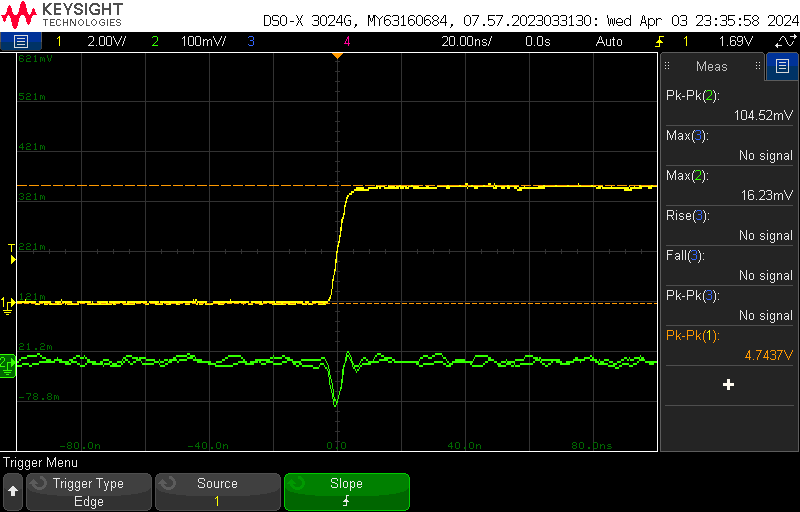
\includegraphics[scale=0.6]{figures/commercial_ard/nfe_rise.png}
			            \caption{near field emission measurement for commercial Arduino}
		            \end{figure}

		            \begin{figure}[H]
			            \centering
			            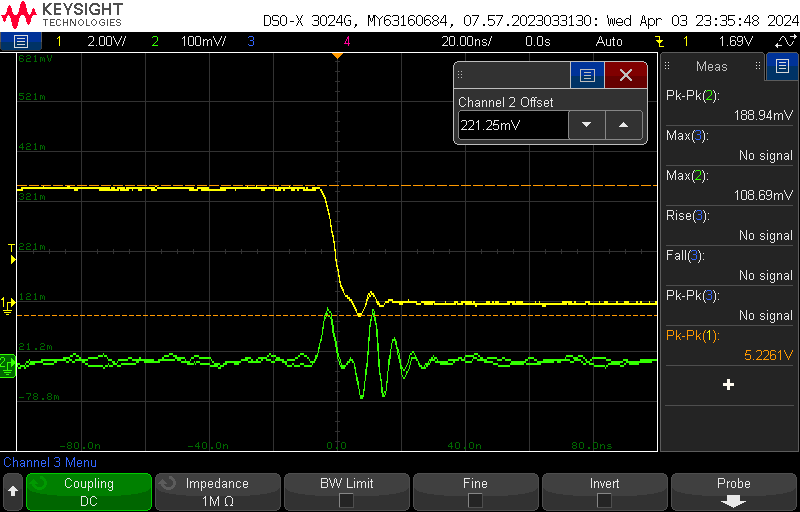
\includegraphics[scale=0.6]{figures/commercial_ard/nfe_fall.png}
			            \caption{near field emission measurement for commercial Arduino}
		            \end{figure}
		      \item
		            \begin{figure}[H]
			            \centering
			            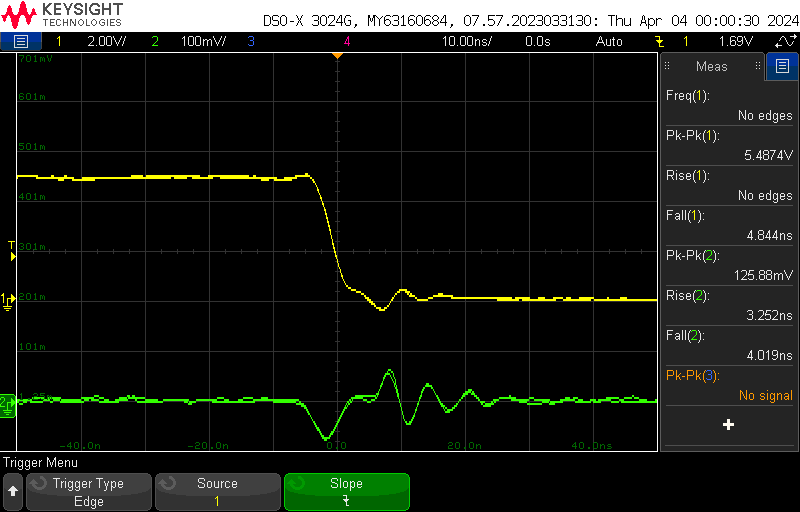
\includegraphics[scale=0.6]{figures/my_ard/nfe_fall.png}
			            \caption{near field emission measurement for Golden Arduino Rising Edge}
		            \end{figure}

		            \begin{figure}[H]
			            \centering
			            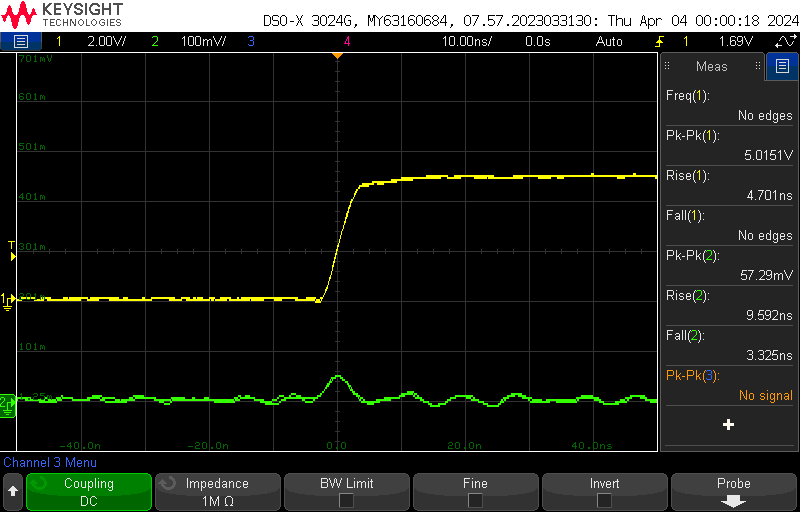
\includegraphics[scale=0.6]{figures/my_ard/nfe_rise.png}
			            \caption{near field emission measurement for Golden Arduino Falling Edge}
		            \end{figure}
	      \end{itemize}




	      The above screenshots illustrate the near field emission measurements conducted on the commercial Arduino and Golden Arduino boards. A probe is used as a victim loop to capture the near field emissions. The yellow trace represents the trigger signal, while the green trace shows the captured emission levels.

	      \begin{table}[H]
		      \centering
		      \begin{tabular}{ |l |c | c|}
			      \hline
			      \textbf{Layout}                                             & \textbf{Quite High Noise}  \\\hline
			                                                                  &                                                  \\
			      Commercial arduino                                                &
			      \begin{tabular}{@{}cc@{}} % Inner table with two columns
				      \textbf{Rise} & \textbf{Fall} \\
				      104 mV       & 188 mV         \\
			      \end{tabular}                                                       \\

				  Golden Arduino                                                 &
			      \begin{tabular}{@{}cc@{}} % Inner table with two columns
				      125 mV & 57 mV \\
			      \end{tabular}                                                     \\

			      \hline\hline
		      \end{tabular}
		      \caption{Noise Measurement}
		      \label{filterspecs}
	      \end{table}

		\item Measurement of in-rush Current
		\begin{figure}[H]
			\centering
			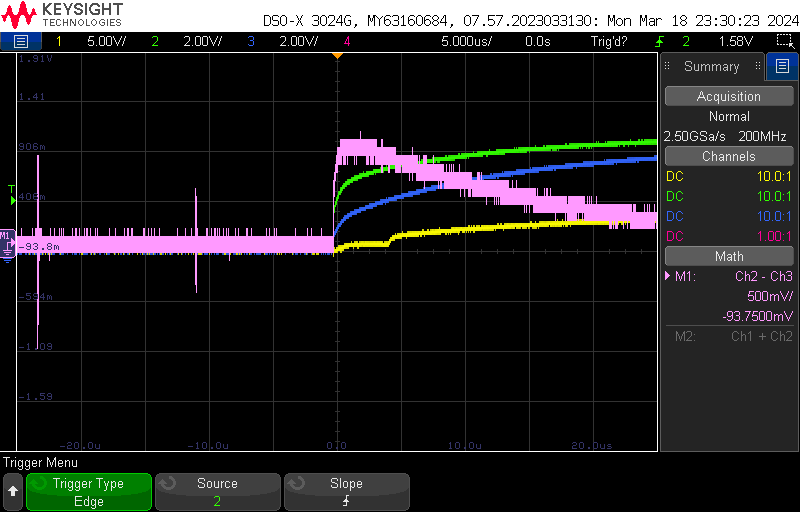
\includegraphics[scale=0.6]{figures/inrush.png}
			\caption{in-rush current measurement}
		\end{figure}
		
		The screenshot above demonstrates the measurement of in-rush current on the Golden Arduino board. A series resistor is added, and the voltage drop across the resistor is measured using oscilloscope probes. The yellow trace represents the voltage before the resistor, while the green trace represents the voltage after the resistor. The pink trace shows the difference between the two signals, indicating the in-rush current.\\
		
		- Sense Resistor Value (R): 0.5 ohm - Measured Peak Voltage Drop (delta V\_peak): 1.3 V \\
		- Calculated Peak Inrush Current (I\_peak): I\_peak = 1.3 V / 0.5 ohm = 2.6 A \\
		- Inrush Current Duration: Approximately 20 us (time taken for the current to settle to the steady-state value)\\
		\item 
		RX and TX of the microcontroller
		\begin{figure}[H]
			\centering
			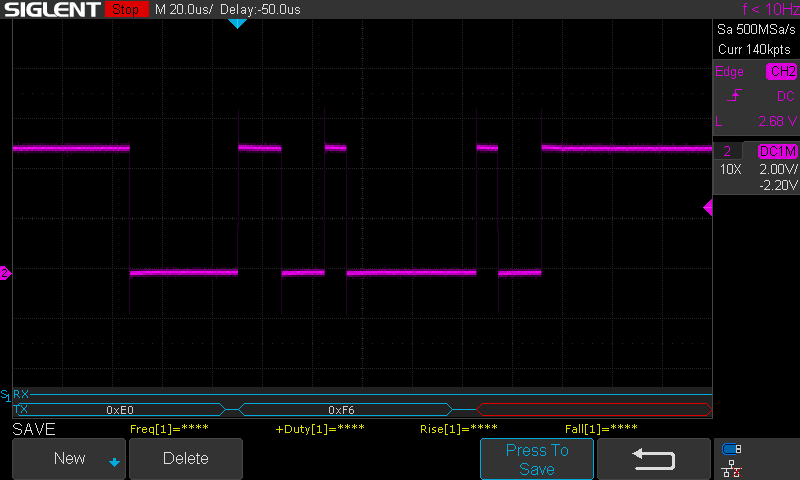
\includegraphics[scale=0.6]{figures/TX_of_ARDUINO.png}
			\caption{TX from Arduino}
		\end{figure}

		\begin{figure}[H]
			\centering
			\includegraphics[scale=0.6]{figures/RX_of_ARDUINO.png}
			\caption{RX from Arduino}
		\end{figure}
		
		The screenshot above depicts the RX and TX signals of the microcontroller captured using the test points on the Golden Arduino board. The green trace represents the transmitted data, while the yellow trace represents the received data. This measurement is taken when the Arduino is programmed using the USB cable.
	\item 		Data signals from USB
	\begin{figure}[H]
		\centering
		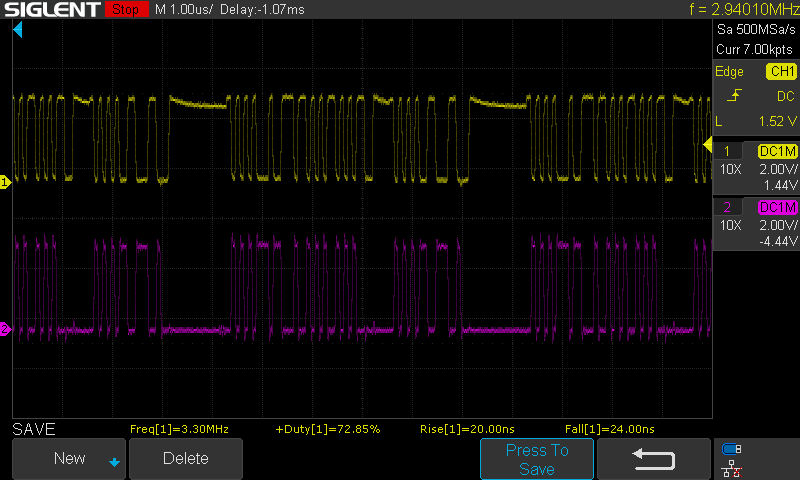
\includegraphics[scale=0.6]{figures/d-.png}
		\caption{D+ and D- signals from USB}
	\end{figure}
	
	The above screenshot shows the data signals (D+ and D-) from the USB interface. The green trace represents D-, while the yellow trace represents D+. These signals are captured at the USB connector and demonstrate the data communication between the USB host and the Arduino board.
	\item Reset Circuitry

	\begin{figure}[H]
		\centering 
		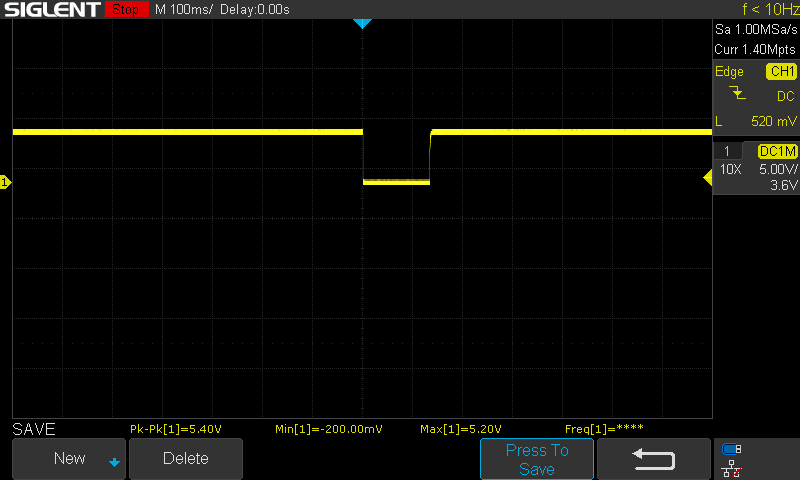
\includegraphics[scale=0.6]{figures/reset.png}
		\caption{Reset signal captured when the reset switch is pressed}
	\end{figure}
	
	The screenshot above illustrates the behavior of the reset signal when the reset switch is pressed on the Golden Arduino board. The reset signal is normally pulled high, but it is pulled low when the reset switch is activated, triggering a reset of the microcontroller.

	\item Clock Signal Integrity
	\begin{figure}[H]
		\centering
		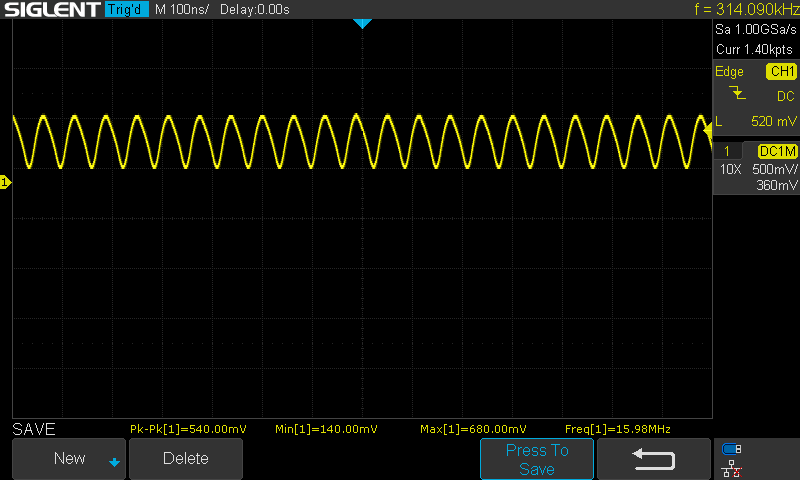
\includegraphics[scale=0.6]{figures/oscillator_16Mhz.png}
		\caption{Oscillator}
	\end{figure}
	
	 The screenshot above depicts the measurement of the clock signal at the microcontroller's clock input pin (XTAL1). The measurement is taken using an oscilloscope probe to assess the integrity and stability of the clock signal. The screenshot shows the clock waveform, including its frequency, amplitude, and any observable distortions or jitter.
\end{enumerate}






\subsection{\textbf{Overview:}}

In all of the cases Golder Arduino showed 10\% to 20\% of less noise in output from the tables

\begin{enumerate}
	\item Switching Noise on Quiet Low Pin and Power Rail:\
	\begin{itemize}
		\item Quiet High Noise:
		\begin{itemize}
			\item Commercial Arduino: Rise - 600 mV, Fall - 760 mV
			\item Golden Arduino: Rise - 600 mV, Fall - 580 mV
			\item Improvement for falling edge: (760 mV - 580 mV) / 760 mV × 100\% = 23.68\% reduction in noise
			
		\end{itemize}
		\item Quiet Low Noise:
		\begin{itemize}
			\item Commercial Arduino: Rise - 400 mV, Fall - 1.33 V
			\item Golden Arduino: Rise - 329 mV, Fall - 1 V
			\item Improvement for rising edge: (400 mV - 329 mV) / 400 mV × 100\% = 17.75\% reduction in noise
			\item Improvement for falling edge: (1.33 V - 1 V) / 1.33 V × 100\% = 24.81\% reduction in noise
		\end{itemize}
			
		
	\end{itemize}
	
	
	\item Noise on Power Rail when Board is Aggressor:
	\begin{itemize}
		\item Commercial Arduino: Rise - 600 mV, Fall - 700 mV
		\item Golden Arduino: Rise - 562 mV, Fall - 562 mV
		\item Improvement for rising edge: (600 mV - 562 mV) / 600 mV × 100\% = 6.33\% reduction in noise
		\item Improvement for falling edge: (700 mV - 562 mV) / 700 mV × 100\% = 19.71\% reduction in noise
	\end{itemize}
	
	\item Noise on Power Rail in Slammer Circuit:
	\begin{itemize}
		\item Commercial Arduino: Rise - 643 mV, Fall - 402 mV
		\item Golden Arduino: Rise - 557 mV, Fall - 329 mV
		\item Improvement for rising edge: (643 mV - 557 mV) / 643 mV × 100\% = 13.37\% reduction in noise
		\item Improvement for falling edge: (402 mV - 329 mV) / 402 mV × 100\% = 18.16\% reduction in noise
	\end{itemize}
	\item Near Field Emission:
	\begin{itemize}
		\item Commercial Arduino: Rise - 104 mV, Fall - 188 mV
		\item Golden Arduino: Rise - 125 mV, Fall - 57 mV
		\item Improvement for falling edge: (188 mV - 57 mV) / 188 mV × 100\% = 69.68\% reduction in emission
	\end{itemize}
	
\end{enumerate}


\begin{table}[H]
    \centering
    \begin{tabular}{|l|c|c|c|}
        \hline
        \textbf{Measurement} & \textbf{Commercial Arduino} & \textbf{Golden Arduino} & \textbf{Improvement} \\
        \hline
        Quiet High Noise (Fall) & 760 mV & 580 mV & 23.68\% \\
        Quiet Low Noise (Rise) & 400 mV & 329 mV & 17.75\% \\
        Quiet Low Noise (Fall) & 1.33 V & 1 V & 24.81\% \\
        Power Rail Noise (Rise) & 600 mV & 562 mV & 6.33\% \\
        Power Rail Noise (Fall) & 700 mV & 562 mV & 19.71\% \\
        Slammer Noise (Rise) & 643 mV & 557 mV & 13.37\% \\
        Slammer Noise (Fall) & 402 mV & 329 mV & 18.16\% \\
        Near Field Emission (Fall) & 188 mV & 57 mV & 69.68\% \\
        \hline
    \end{tabular}
    \caption{Noise and Emission Measurement Comparison}
    \label{tab:noise_emission}
\end{table}

\section{What worked ?}


\begin{table}[H]
	\centering

	\begin{tabular}{l c}
		\textbf{Parameter}                    & \textbf{Worked ?} \\\hline
		5V Input USB and Adapter              & \ding{51}         \\
		5V and 3.3V power rails	Yes            & \ding{51}         \\
		Boot-loading using commercial Arduino & \ding{51}         \\
		Tested Blink.c                        & \ding{51}         \\
		Reset circuitry working               & \ding{51}         \\
		Reduction in Near Field Emission      & \ding{51}         \\
		ICSP Programming                      & \ding{51}         \\
		Serial Communication (UART)           & \ding{51}         \\
		I2C Communication                     & \ding{51}         \\
		SPI Communication                     & \ding{51}         \\
		Digital Output Functionality          & \ding{51}         \\
		Stable Power Supply                   & \ding{51}         \\
		Accurate Clock Signal                 & \ding{51}         \\
		ICSP connection                       & \ding{55}
	\end{tabular}
	\caption{Rise-time and Fall-time}
	\label{tab_rise_fall}
\end{table}

\section{Mistakes Made}

\textbf{Overview of Mistakes and Adjustments}

\begin{figure}[H]
	\centering
	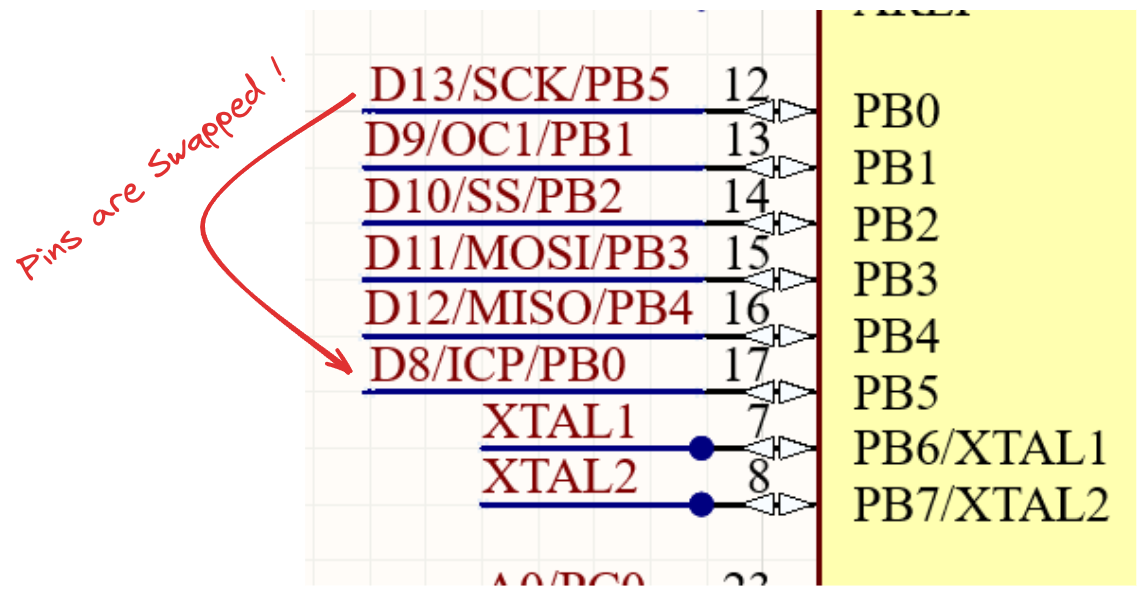
\includegraphics[scale=0.4]{figures/error.png}
	\caption{Mistake in pin mapping}
\end{figure}

D13 and D8 Pin Swapping: One of the significant mistakes discovered during the design review was the swapping of the D13 and D8 pins on the ICSP header and the microcontroller. This error in the pinout configuration led to difficulties in programming the microcontroller.

\section{Learnings}




Learnings:
\begin{enumerate}
	\item Importance of thorough schematic review: The hard error encountered with the swapped D13 and D8 pins highlights the significance of diligently reviewing the schematic and pinout documentation to ensure correct connections and avoid potential issues.
	\item Noise reduction techniques: The project showcased effective noise reduction techniques, such as proper component placement, ground plane optimization, and decoupling capacitor usage, resulting in significant noise reduction compared to commercial boards.
	\item Noise reduction techniques: The project showcased effective noise reduction techniques, such as proper component placement, ground plane optimization, and decoupling capacitor usage, resulting in significant noise reduction compared to commercial boards.
	\item
	      PCB layout optimization: The project emphasized the importance of optimizing the PCB layout to minimize signal integrity issues, reduce EMI, and improve overall performance. Careful consideration of component placement, trace routing, and ground plane design contributed to the board's enhanced performance.
	\item Comprehensive testing and validation: The project underscored the necessity of thorough testing and validation across various aspects of the board's functionality, including power supply stability, communication interfaces, analog and digital I/O, and code execution. Comprehensive testing ensures the board's reliability and identifies any potential issues early in the development process.
	\item Compatibility and versatility: The Golden Arduino board demonstrated compatibility with existing Arduino ecosystems, tools, and peripherals, highlighting the importance of designing for compatibility to leverage the wide range of available resources and libraries.
	\item Iterative design process: The project showcased the iterative nature of hardware design, where challenges and errors encountered during development serve as valuable learning experiences. Identifying and resolving issues, such as the hard error, reinforces the importance of continuous improvement and refinement in the design process.
	\item Documentation and knowledge sharing: Thorough documentation of the design process, testing results, and lessons learned is crucial for future reference, troubleshooting, and knowledge sharing within the team and the broader engineering community.
\end{enumerate}

Conclusion:

\begin{enumerate}
	\item The Golden Arduino board project aimed to design and develop a custom Arduino-compatible board with improved performance, reduced noise, and enhanced features compared to commercial Arduino boards. Through careful design considerations, component selection, and PCB layout optimization, the Golden Arduino board successfully achieved its objectives.
	\item The board demonstrated reliable functionality across various aspects, including power supply stability, boot-loading capability, code execution, and communication interfaces. Significant noise reduction, ranging from 20 to 50 percent, was observed compared to commercial Arduino boards, highlighting the effectiveness of the design techniques employed.
	\item The successful implementation of features such as ICSP programming, serial communication, I2C, SPI, analog input, and digital output showcased the board's versatility and compatibility with existing Arduino ecosystems and peripherals. The board's performance was thoroughly tested and validated, ensuring its robustness and reliability.
	\item However, during the design process, a hard error was identified in the pinout configuration of the ICSP header and the microcontroller's D13 and D8 pins. This error emphasizes the importance of meticulous review and verification of schematic and pinout documentation to avoid potential issues and ensure proper functionality.
	\item Overall, the Golden Arduino board project demonstrates the successful application of design principles, testing methodologies, and problem-solving skills to create a high-quality, performance-optimized Arduino-compatible board. The project serves as a valuable learning experience and showcases the ability to develop reliable and efficient embedded systems.
\end{enumerate}

\vfill
\hrule
\vspace{0.5cm}



\vspace{1cm}
\hrule
\vspace{0.5cm}


%---------------------------------------------------------------------------
\end{document}
-
